% Options for packages loaded elsewhere
\PassOptionsToPackage{unicode}{hyperref}
\PassOptionsToPackage{hyphens}{url}
%
\documentclass[
]{article}
\usepackage{amsmath,amssymb}
\usepackage{iftex}
\ifPDFTeX
  \usepackage[T1]{fontenc}
  \usepackage[utf8]{inputenc}
  \usepackage{textcomp} % provide euro and other symbols
\else % if luatex or xetex
  \usepackage{unicode-math} % this also loads fontspec
  \defaultfontfeatures{Scale=MatchLowercase}
  \defaultfontfeatures[\rmfamily]{Ligatures=TeX,Scale=1}
\fi
\usepackage{lmodern}
\ifPDFTeX\else
  % xetex/luatex font selection
  \setmainfont[]{Linux Libertine}
\fi
% Use upquote if available, for straight quotes in verbatim environments
\IfFileExists{upquote.sty}{\usepackage{upquote}}{}
\IfFileExists{microtype.sty}{% use microtype if available
  \usepackage[]{microtype}
  \UseMicrotypeSet[protrusion]{basicmath} % disable protrusion for tt fonts
}{}
\makeatletter
\@ifundefined{KOMAClassName}{% if non-KOMA class
  \IfFileExists{parskip.sty}{%
    \usepackage{parskip}
  }{% else
    \setlength{\parindent}{0pt}
    \setlength{\parskip}{6pt plus 2pt minus 1pt}}
}{% if KOMA class
  \KOMAoptions{parskip=half}}
\makeatother
\usepackage{xcolor}
\usepackage[margin=1in]{geometry}
\usepackage{color}
\usepackage{fancyvrb}
\newcommand{\VerbBar}{|}
\newcommand{\VERB}{\Verb[commandchars=\\\{\}]}
\DefineVerbatimEnvironment{Highlighting}{Verbatim}{commandchars=\\\{\}}
% Add ',fontsize=\small' for more characters per line
\usepackage{framed}
\definecolor{shadecolor}{RGB}{248,248,248}
\newenvironment{Shaded}{\begin{snugshade}}{\end{snugshade}}
\newcommand{\AlertTok}[1]{\textcolor[rgb]{0.94,0.16,0.16}{#1}}
\newcommand{\AnnotationTok}[1]{\textcolor[rgb]{0.56,0.35,0.01}{\textbf{\textit{#1}}}}
\newcommand{\AttributeTok}[1]{\textcolor[rgb]{0.13,0.29,0.53}{#1}}
\newcommand{\BaseNTok}[1]{\textcolor[rgb]{0.00,0.00,0.81}{#1}}
\newcommand{\BuiltInTok}[1]{#1}
\newcommand{\CharTok}[1]{\textcolor[rgb]{0.31,0.60,0.02}{#1}}
\newcommand{\CommentTok}[1]{\textcolor[rgb]{0.56,0.35,0.01}{\textit{#1}}}
\newcommand{\CommentVarTok}[1]{\textcolor[rgb]{0.56,0.35,0.01}{\textbf{\textit{#1}}}}
\newcommand{\ConstantTok}[1]{\textcolor[rgb]{0.56,0.35,0.01}{#1}}
\newcommand{\ControlFlowTok}[1]{\textcolor[rgb]{0.13,0.29,0.53}{\textbf{#1}}}
\newcommand{\DataTypeTok}[1]{\textcolor[rgb]{0.13,0.29,0.53}{#1}}
\newcommand{\DecValTok}[1]{\textcolor[rgb]{0.00,0.00,0.81}{#1}}
\newcommand{\DocumentationTok}[1]{\textcolor[rgb]{0.56,0.35,0.01}{\textbf{\textit{#1}}}}
\newcommand{\ErrorTok}[1]{\textcolor[rgb]{0.64,0.00,0.00}{\textbf{#1}}}
\newcommand{\ExtensionTok}[1]{#1}
\newcommand{\FloatTok}[1]{\textcolor[rgb]{0.00,0.00,0.81}{#1}}
\newcommand{\FunctionTok}[1]{\textcolor[rgb]{0.13,0.29,0.53}{\textbf{#1}}}
\newcommand{\ImportTok}[1]{#1}
\newcommand{\InformationTok}[1]{\textcolor[rgb]{0.56,0.35,0.01}{\textbf{\textit{#1}}}}
\newcommand{\KeywordTok}[1]{\textcolor[rgb]{0.13,0.29,0.53}{\textbf{#1}}}
\newcommand{\NormalTok}[1]{#1}
\newcommand{\OperatorTok}[1]{\textcolor[rgb]{0.81,0.36,0.00}{\textbf{#1}}}
\newcommand{\OtherTok}[1]{\textcolor[rgb]{0.56,0.35,0.01}{#1}}
\newcommand{\PreprocessorTok}[1]{\textcolor[rgb]{0.56,0.35,0.01}{\textit{#1}}}
\newcommand{\RegionMarkerTok}[1]{#1}
\newcommand{\SpecialCharTok}[1]{\textcolor[rgb]{0.81,0.36,0.00}{\textbf{#1}}}
\newcommand{\SpecialStringTok}[1]{\textcolor[rgb]{0.31,0.60,0.02}{#1}}
\newcommand{\StringTok}[1]{\textcolor[rgb]{0.31,0.60,0.02}{#1}}
\newcommand{\VariableTok}[1]{\textcolor[rgb]{0.00,0.00,0.00}{#1}}
\newcommand{\VerbatimStringTok}[1]{\textcolor[rgb]{0.31,0.60,0.02}{#1}}
\newcommand{\WarningTok}[1]{\textcolor[rgb]{0.56,0.35,0.01}{\textbf{\textit{#1}}}}
\usepackage{longtable,booktabs,array}
\usepackage{calc} % for calculating minipage widths
% Correct order of tables after \paragraph or \subparagraph
\usepackage{etoolbox}
\makeatletter
\patchcmd\longtable{\par}{\if@noskipsec\mbox{}\fi\par}{}{}
\makeatother
% Allow footnotes in longtable head/foot
\IfFileExists{footnotehyper.sty}{\usepackage{footnotehyper}}{\usepackage{footnote}}
\makesavenoteenv{longtable}
\usepackage{graphicx}
\makeatletter
\def\maxwidth{\ifdim\Gin@nat@width>\linewidth\linewidth\else\Gin@nat@width\fi}
\def\maxheight{\ifdim\Gin@nat@height>\textheight\textheight\else\Gin@nat@height\fi}
\makeatother
% Scale images if necessary, so that they will not overflow the page
% margins by default, and it is still possible to overwrite the defaults
% using explicit options in \includegraphics[width, height, ...]{}
\setkeys{Gin}{width=\maxwidth,height=\maxheight,keepaspectratio}
% Set default figure placement to htbp
\makeatletter
\def\fps@figure{htbp}
\makeatother
\setlength{\emergencystretch}{3em} % prevent overfull lines
\providecommand{\tightlist}{%
  \setlength{\itemsep}{0pt}\setlength{\parskip}{0pt}}
\setcounter{secnumdepth}{-\maxdimen} % remove section numbering
% definitions for citeproc citations
\NewDocumentCommand\citeproctext{}{}
\NewDocumentCommand\citeproc{mm}{%
  \begingroup\def\citeproctext{#2}\cite{#1}\endgroup}
\makeatletter
 % allow citations to break across lines
 \let\@cite@ofmt\@firstofone
 % avoid brackets around text for \cite:
 \def\@biblabel#1{}
 \def\@cite#1#2{{#1\if@tempswa , #2\fi}}
\makeatother
\newlength{\cslhangindent}
\setlength{\cslhangindent}{1.5em}
\newlength{\csllabelwidth}
\setlength{\csllabelwidth}{3em}
\newenvironment{CSLReferences}[2] % #1 hanging-indent, #2 entry-spacing
 {\begin{list}{}{%
  \setlength{\itemindent}{0pt}
  \setlength{\leftmargin}{0pt}
  \setlength{\parsep}{0pt}
  % turn on hanging indent if param 1 is 1
  \ifodd #1
   \setlength{\leftmargin}{\cslhangindent}
   \setlength{\itemindent}{-1\cslhangindent}
  \fi
  % set entry spacing
  \setlength{\itemsep}{#2\baselineskip}}}
 {\end{list}}
\usepackage{calc}
\newcommand{\CSLBlock}[1]{\hfill\break\parbox[t]{\linewidth}{\strut\ignorespaces#1\strut}}
\newcommand{\CSLLeftMargin}[1]{\parbox[t]{\csllabelwidth}{\strut#1\strut}}
\newcommand{\CSLRightInline}[1]{\parbox[t]{\linewidth - \csllabelwidth}{\strut#1\strut}}
\newcommand{\CSLIndent}[1]{\hspace{\cslhangindent}#1}
\usepackage{fvextra}
\DefineVerbatimEnvironment{Highlighting}{Verbatim}{
  breaksymbolleft={}, 
  showspaces = false,
  showtabs = false,
  breaklines,
  commandchars=\\\{\}
}

\usepackage{booktabs}
\usepackage{longtable}
\usepackage{array}
\usepackage{multirow}
\usepackage{wrapfig}
\usepackage{float}
\usepackage{colortbl}
\usepackage{pdflscape}
\usepackage{tabu}
\usepackage{threeparttable}
\usepackage{threeparttablex}
\usepackage[normalem]{ulem}
\usepackage{makecell}
\usepackage{xcolor}
\ifLuaTeX
  \usepackage{selnolig}  % disable illegal ligatures
\fi
\usepackage{bookmark}
\IfFileExists{xurl.sty}{\usepackage{xurl}}{} % add URL line breaks if available
\urlstyle{same}
\hypersetup{
  pdftitle={Analyses and plots for Chapter 17 -- Discussion},
  pdfauthor={Sandra Auderset},
  hidelinks,
  pdfcreator={LaTeX via pandoc}}

\title{Analyses and plots for Chapter 17 -- Discussion}
\usepackage{etoolbox}
\makeatletter
\providecommand{\subtitle}[1]{% add subtitle to \maketitle
  \apptocmd{\@title}{\par {\large #1 \par}}{}{}
}
\makeatother
\subtitle{Constituency and convergence in the Americas}
\author{Sandra Auderset}
\date{16 July, 2024}

\begin{document}
\maketitle

{
\setcounter{tocdepth}{2}
\tableofcontents
}
This script provides all the code for the analyses and figures presented
in the discussion chapter (17) in the order of the chapter text.

\section{Section 3}\label{section-3}

\subsection{Map of the sample
languages}\label{map-of-the-sample-languages}

Create map of the sample languages. This includes all the languages
which are discussed in the chapters of the volume, Chacobo, which was
discussed in (\textbf{tallman2021constituency?}), and Siksika, which
could not be included in the first volume but is fully analyzed (Natalie
Weber, p.c.). The map is created using Stadia Maps (stadiamaps.com) with
ggmaps Kahle \& Wickham (2013).

\begin{Shaded}
\begin{Highlighting}[]
\CommentTok{\# read in constituency database}
\NormalTok{domains }\OtherTok{\textless{}{-}} \FunctionTok{read\_tsv}\NormalTok{(}\FunctionTok{here}\NormalTok{(}\StringTok{"domains.tsv"}\NormalTok{)) }\SpecialCharTok{\%\textgreater{}\%}
  \FunctionTok{modify\_if}\NormalTok{(is.character, as.factor)}
\end{Highlighting}
\end{Shaded}

\begin{verbatim}
## Rows: 463 Columns: 21
## -- Column specification --------------------------------------------------------
## Delimiter: "\t"
## chr (11): Language_Name, Language_ID, Domain_ID, Domain_Type, Abstract_Type,...
## dbl (10): Serial_Order, Left_Edge, Right_Edge, Convergence, Relative_Converg...
## 
## i Use `spec()` to retrieve the full column specification for this data.
## i Specify the column types or set `show_col_types = FALSE` to quiet this message.
\end{verbatim}

\begin{Shaded}
\begin{Highlighting}[]
\CommentTok{\# read in metadata file}
\NormalTok{metadata }\OtherTok{\textless{}{-}} \FunctionTok{read\_tsv}\NormalTok{(}\FunctionTok{here}\NormalTok{(}\StringTok{"input/metadata.tsv"}\NormalTok{))}
\end{Highlighting}
\end{Shaded}

\begin{verbatim}
## Rows: 37 Columns: 10
## -- Column specification --------------------------------------------------------
## Delimiter: "\t"
## chr (7): Language_Name, Alternative_Name, Short_Name, Language_ID, Glottocod...
## dbl (3): No, Latitude, Longitude
## 
## i Use `spec()` to retrieve the full column specification for this data.
## i Specify the column types or set `show_col_types = FALSE` to quiet this message.
\end{verbatim}

\begin{Shaded}
\begin{Highlighting}[]
\CommentTok{\# subset for languages of volume 1 and Chacobo and Siksika}
\NormalTok{metadata\_sub }\OtherTok{\textless{}{-}}\NormalTok{ metadata }\SpecialCharTok{\%\textgreater{}\%}
  \FunctionTok{filter}\NormalTok{(Contribution }\SpecialCharTok{==} \StringTok{"Vol1"} \SpecialCharTok{|}\NormalTok{ Language\_ID }\SpecialCharTok{==} \StringTok{"siks1238"} \SpecialCharTok{|}\NormalTok{ Language\_ID }\SpecialCharTok{==} \StringTok{"chac1251"}\NormalTok{)}

\CommentTok{\# find min/max values of lat and long for map}
\FunctionTok{summary}\NormalTok{(metadata\_sub}\SpecialCharTok{$}\NormalTok{Latitude)}
\end{Highlighting}
\end{Shaded}

\begin{verbatim}
##    Min. 1st Qu.  Median    Mean 3rd Qu.    Max. 
##  -28.10  -12.13   14.64    9.60   18.10   60.31
\end{verbatim}

\begin{Shaded}
\begin{Highlighting}[]
\FunctionTok{summary}\NormalTok{(metadata\_sub}\SpecialCharTok{$}\NormalTok{Longitude)}
\end{Highlighting}
\end{Shaded}

\begin{verbatim}
##    Min. 1st Qu.  Median    Mean 3rd Qu.    Max. 
## -161.49  -97.46  -71.00  -83.71  -66.17  -51.67
\end{verbatim}

\begin{Shaded}
\begin{Highlighting}[]
\CommentTok{\# get basemap}
\NormalTok{americas }\OtherTok{\textless{}{-}} \FunctionTok{get\_stadiamap}\NormalTok{(}\AttributeTok{bbox =} \FunctionTok{c}\NormalTok{(}\AttributeTok{left =} \SpecialCharTok{{-}}\DecValTok{167}\NormalTok{, }\AttributeTok{bottom =} \SpecialCharTok{{-}}\DecValTok{36}\NormalTok{, }\AttributeTok{right =} \SpecialCharTok{{-}}\DecValTok{40}\NormalTok{, }\AttributeTok{top =} \DecValTok{64}\NormalTok{), }\AttributeTok{maptype =} \StringTok{"stamen\_terrain"}\NormalTok{, }\AttributeTok{zoom =} \DecValTok{5}\NormalTok{)}
\end{Highlighting}
\end{Shaded}

\begin{verbatim}
## i © Stadia Maps © Stamen Design © OpenMapTiles © OpenStreetMap contributors.
## i 144 tiles needed, this may take a while (try a smaller zoom?)
\end{verbatim}

\begin{Shaded}
\begin{Highlighting}[]
\CommentTok{\# add points for languages}
\NormalTok{sample\_map }\OtherTok{\textless{}{-}} \FunctionTok{ggmap}\NormalTok{(americas) }\SpecialCharTok{+}
  \FunctionTok{geom\_point}\NormalTok{(}\FunctionTok{aes}\NormalTok{(}\AttributeTok{x =}\NormalTok{ Longitude, }\AttributeTok{y =}\NormalTok{ Latitude), }\AttributeTok{data =}\NormalTok{ metadata\_sub, }\AttributeTok{alpha =} \DecValTok{1}\NormalTok{, }\AttributeTok{size =} \DecValTok{3}\NormalTok{) }\SpecialCharTok{+}
  \FunctionTok{geom\_label\_repel}\NormalTok{(}\FunctionTok{aes}\NormalTok{(}\AttributeTok{x =}\NormalTok{ Longitude, }\AttributeTok{y =}\NormalTok{ Latitude, }\AttributeTok{label =}\NormalTok{ Short\_Name), }\AttributeTok{data =}\NormalTok{ metadata\_sub, }\AttributeTok{box.padding =} \FunctionTok{unit}\NormalTok{(.}\DecValTok{3}\NormalTok{, }\StringTok{"lines"}\NormalTok{), }\AttributeTok{label.padding =} \FunctionTok{unit}\NormalTok{(.}\DecValTok{2}\NormalTok{, }\StringTok{"lines"}\NormalTok{), }\AttributeTok{max.overlaps =} \DecValTok{30}\NormalTok{, }\AttributeTok{size =} \DecValTok{3}\NormalTok{) }\SpecialCharTok{+}
  \FunctionTok{theme\_map}\NormalTok{()}
\NormalTok{sample\_map}
\end{Highlighting}
\end{Shaded}

\begin{center}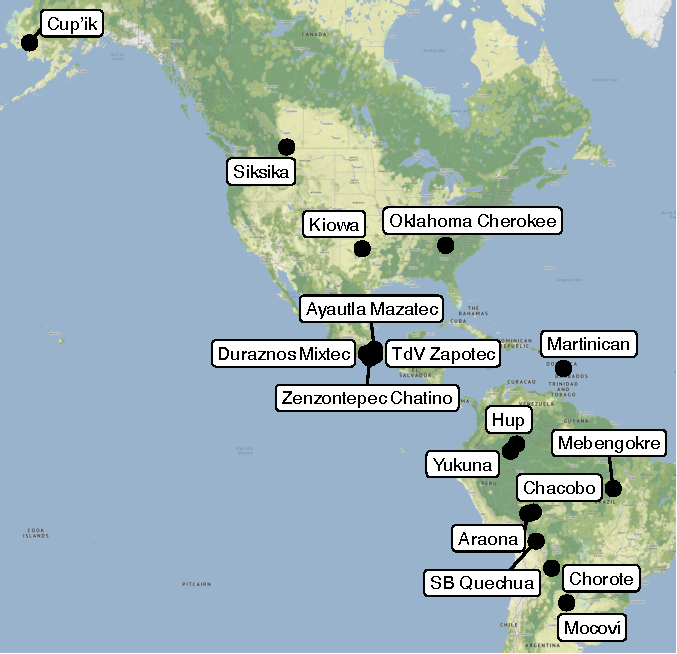
\includegraphics[width=0.9\textwidth,height=\textheight]{02_analyses_chapter17_files/figure-latex/map prep-1} \end{center}

We color the points by maximum number of relative convergences per
language.

\begin{Shaded}
\begin{Highlighting}[]
\CommentTok{\# merge with domains file}
\NormalTok{metadata\_sub\_conv }\OtherTok{\textless{}{-}}\NormalTok{ domains }\SpecialCharTok{\%\textgreater{}\%}
  \FunctionTok{select}\NormalTok{(Language\_ID, Relative\_Convergence) }\SpecialCharTok{\%\textgreater{}\%}
  \FunctionTok{group\_by}\NormalTok{(Language\_ID) }\SpecialCharTok{\%\textgreater{}\%}
  \FunctionTok{slice}\NormalTok{(}\FunctionTok{which.max}\NormalTok{(Relative\_Convergence)) }\SpecialCharTok{\%\textgreater{}\%}
  \FunctionTok{left\_join}\NormalTok{(., metadata\_sub)}
\end{Highlighting}
\end{Shaded}

\begin{verbatim}
## Joining with `by = join_by(Language_ID)`
\end{verbatim}

\begin{Shaded}
\begin{Highlighting}[]
\CommentTok{\# update map}
\NormalTok{sample\_map\_relconv }\OtherTok{\textless{}{-}} \FunctionTok{ggmap}\NormalTok{(americas) }\SpecialCharTok{+}
  \FunctionTok{geom\_point}\NormalTok{(}\FunctionTok{aes}\NormalTok{(}\AttributeTok{x =}\NormalTok{ Longitude, }\AttributeTok{y =}\NormalTok{ Latitude, }\AttributeTok{fill =}\NormalTok{ Relative\_Convergence), }\AttributeTok{data =}\NormalTok{ metadata\_sub\_conv, }\AttributeTok{size =} \DecValTok{4}\NormalTok{, }\AttributeTok{pch =} \DecValTok{21}\NormalTok{) }\SpecialCharTok{+}
  \FunctionTok{scale\_fill\_viridis}\NormalTok{(}
    \AttributeTok{option =} \StringTok{"inferno"}\NormalTok{, }\AttributeTok{direction =} \SpecialCharTok{{-}}\DecValTok{1}\NormalTok{, }\AttributeTok{end =} \FloatTok{0.9}\NormalTok{,}
    \AttributeTok{name =} \StringTok{"Max. Relative Convergence"}\NormalTok{,}
    \AttributeTok{breaks =} \FunctionTok{seq}\NormalTok{(}\DecValTok{0}\NormalTok{, }\FloatTok{0.45}\NormalTok{, }\AttributeTok{by =} \FloatTok{0.05}\NormalTok{)}
\NormalTok{  ) }\SpecialCharTok{+}
  \FunctionTok{geom\_label\_repel}\NormalTok{(}\FunctionTok{aes}\NormalTok{(}\AttributeTok{x =}\NormalTok{ Longitude, }\AttributeTok{y =}\NormalTok{ Latitude, }\AttributeTok{label =}\NormalTok{ Short\_Name), }\AttributeTok{data =}\NormalTok{ metadata\_sub, }\AttributeTok{box.padding =}\NormalTok{ .}\DecValTok{6}\NormalTok{, }\AttributeTok{point.padding =} \DecValTok{1}\NormalTok{, }\AttributeTok{max.overlaps =} \DecValTok{30}\NormalTok{, }\AttributeTok{min.segment.length =} \FloatTok{0.1}\NormalTok{, }\AttributeTok{size =} \DecValTok{5}\NormalTok{) }\SpecialCharTok{+}
  \FunctionTok{theme\_map}\NormalTok{() }\SpecialCharTok{+}
  \FunctionTok{theme}\NormalTok{(}
    \AttributeTok{legend.position =} \FunctionTok{c}\NormalTok{(}\FloatTok{0.05}\NormalTok{, }\FloatTok{0.05}\NormalTok{),}
    \AttributeTok{legend.direction =} \StringTok{"vertical"}\NormalTok{,}
    \AttributeTok{legend.title =} \FunctionTok{element\_text}\NormalTok{(}\AttributeTok{size =} \DecValTok{12}\NormalTok{),}
    \AttributeTok{legend.text =} \FunctionTok{element\_text}\NormalTok{(}\AttributeTok{size =} \DecValTok{12}\NormalTok{)}
\NormalTok{  )}
\NormalTok{sample\_map\_relconv}
\end{Highlighting}
\end{Shaded}

\begin{center}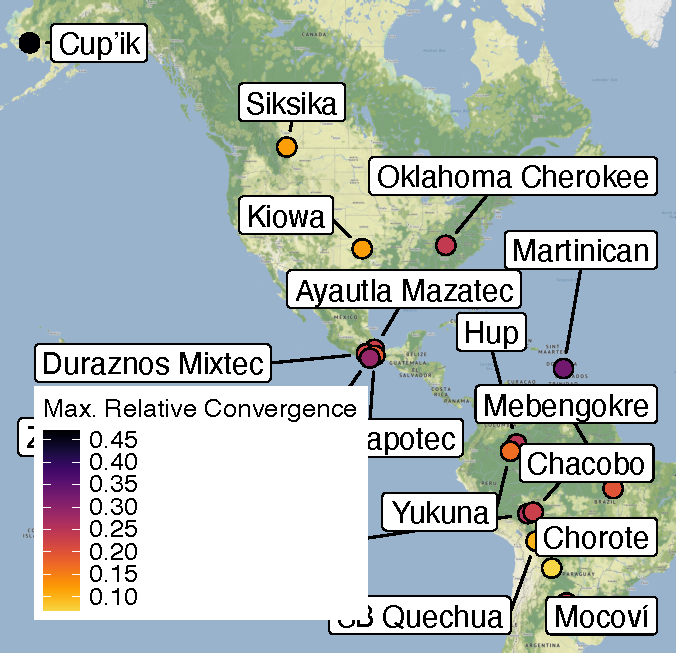
\includegraphics[width=0.9\textwidth,height=\textheight]{02_analyses_chapter17_files/figure-latex/map convergences-1} \end{center}

\subsection{Dot plot of convergences and span
size}\label{dot-plot-of-convergences-and-span-size}

We plot the relative convergences against the relative span size per
sample language. We use only verbal domains as we currently have too
little data for comparing nominal domains as well.

\begin{Shaded}
\begin{Highlighting}[]
\CommentTok{\# exclude all domains that are not verbal; add short name of languages for plotting}
\NormalTok{domains\_verbal }\OtherTok{\textless{}{-}}\NormalTok{ domains }\SpecialCharTok{\%\textgreater{}\%}
  \FunctionTok{filter}\NormalTok{(}\FunctionTok{str\_detect}\NormalTok{(Planar\_ID, }\StringTok{"verbal"}\NormalTok{)) }\SpecialCharTok{\%\textgreater{}\%}
  \FunctionTok{filter}\NormalTok{(}\SpecialCharTok{!}\FunctionTok{is.na}\NormalTok{(Convergence)) }\SpecialCharTok{\%\textgreater{}\%}
  \FunctionTok{left\_join}\NormalTok{(., }\FunctionTok{select}\NormalTok{(metadata\_sub, Language\_ID, Short\_Name)) }\SpecialCharTok{\%\textgreater{}\%}
  \FunctionTok{arrange}\NormalTok{(Relative\_Size, Relative\_Convergence)}
\end{Highlighting}
\end{Shaded}

\begin{verbatim}
## Joining with `by = join_by(Language_ID)`
\end{verbatim}

\begin{Shaded}
\begin{Highlighting}[]
\CommentTok{\# make dot plot per language}
\NormalTok{plot\_rconv\_facet }\OtherTok{\textless{}{-}} \FunctionTok{ggplot}\NormalTok{(}\FunctionTok{aes}\NormalTok{(}\AttributeTok{x =}\NormalTok{ Relative\_Size, }\AttributeTok{y =}\NormalTok{ Relative\_Convergence, }\AttributeTok{group =}\NormalTok{ Language\_Name), }\AttributeTok{data =}\NormalTok{ domains\_verbal) }\SpecialCharTok{+}
  \FunctionTok{geom\_point}\NormalTok{(}\FunctionTok{aes}\NormalTok{(), }\AttributeTok{size =} \FloatTok{2.5}\NormalTok{) }\SpecialCharTok{+}
  \FunctionTok{geom\_line}\NormalTok{(}\AttributeTok{linewidth =} \FloatTok{0.5}\NormalTok{) }\SpecialCharTok{+}
  \FunctionTok{facet\_wrap}\NormalTok{(}\SpecialCharTok{\textasciitilde{}}\NormalTok{Short\_Name, }\AttributeTok{nrow =} \DecValTok{6}\NormalTok{, }\AttributeTok{ncol =} \DecValTok{3}\NormalTok{, }\AttributeTok{scales =} \StringTok{"free\_x"}\NormalTok{) }\SpecialCharTok{+}
  \FunctionTok{ylab}\NormalTok{(}\StringTok{"Relative convergences"}\NormalTok{) }\SpecialCharTok{+}
  \FunctionTok{xlab}\NormalTok{(}\StringTok{"Relative span size"}\NormalTok{) }\SpecialCharTok{+}
  \FunctionTok{scale\_x\_continuous}\NormalTok{(}\AttributeTok{limits =} \FunctionTok{c}\NormalTok{(}\DecValTok{0}\NormalTok{, }\DecValTok{1}\NormalTok{), }\AttributeTok{breaks =} \FunctionTok{seq}\NormalTok{(}\DecValTok{0}\NormalTok{, }\DecValTok{1}\NormalTok{, }\FloatTok{0.25}\NormalTok{)) }\SpecialCharTok{+}
  \FunctionTok{scale\_y\_continuous}\NormalTok{(}\AttributeTok{limits =} \FunctionTok{c}\NormalTok{(}\DecValTok{0}\NormalTok{, }\FloatTok{0.5}\NormalTok{)) }\SpecialCharTok{+}
  \FunctionTok{theme\_bw}\NormalTok{() }\SpecialCharTok{+}
  \FunctionTok{theme}\NormalTok{(}
    \AttributeTok{axis.text =} \FunctionTok{element\_text}\NormalTok{(}\AttributeTok{size =} \DecValTok{11}\NormalTok{),}
    \AttributeTok{axis.title =} \FunctionTok{element\_text}\NormalTok{(}\AttributeTok{size =} \DecValTok{12}\NormalTok{),}
    \AttributeTok{strip.text.x =} \FunctionTok{element\_text}\NormalTok{(}\AttributeTok{size =} \DecValTok{11}\NormalTok{),}
    \AttributeTok{panel.spacing =} \FunctionTok{unit}\NormalTok{(}\FloatTok{1.2}\NormalTok{, }\StringTok{"lines"}\NormalTok{)}
\NormalTok{  )}
\NormalTok{plot\_rconv\_facet}
\end{Highlighting}
\end{Shaded}

\begin{center}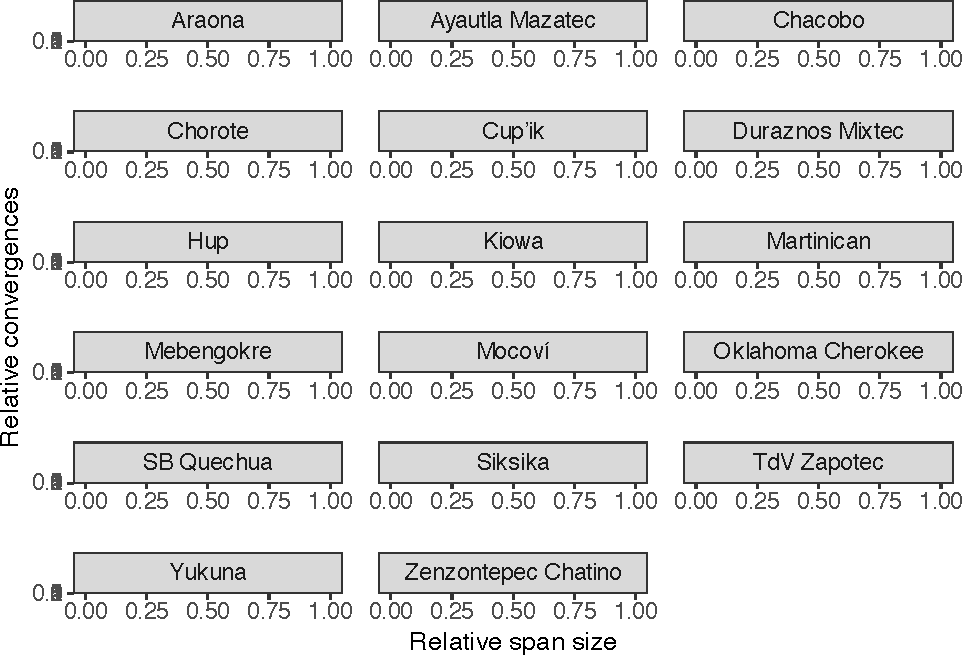
\includegraphics[width=0.9\textwidth,height=\textheight]{02_analyses_chapter17_files/figure-latex/dot plot-1} \end{center}

\subsection{Density plot of span size by
type}\label{density-plot-of-span-size-by-type}

We plot densities of relative span size by abstract type of test domain.
Since we are doing this across languages, we exclude abstract types that
have less than 10 data points, as these are not informative.

\begin{Shaded}
\begin{Highlighting}[]
\CommentTok{\# list all abstract types}
\FunctionTok{levels}\NormalTok{(domains}\SpecialCharTok{$}\NormalTok{Abstract\_Type)}
\end{Highlighting}
\end{Shaded}

\begin{verbatim}
##  [1] "ciscategorial.selection" "deviations"             
##  [3] "free.occurrence"         "idiom"                  
##  [5] "noninterruption"         "nonpermutability"       
##  [7] "pausing"                 "play.language"          
##  [9] "proform"                 "recursion.based"        
## [11] "repair"                  "segmental"              
## [13] "suprasegmental"
\end{verbatim}

\begin{Shaded}
\begin{Highlighting}[]
\CommentTok{\# remove types with under 10 data points}
\NormalTok{include\_at }\OtherTok{\textless{}{-}}\NormalTok{ domains\_verbal }\SpecialCharTok{\%\textgreater{}\%}
  \FunctionTok{count}\NormalTok{(Abstract\_Type) }\SpecialCharTok{\%\textgreater{}\%}
  \FunctionTok{arrange}\NormalTok{(}\FunctionTok{desc}\NormalTok{(n)) }\SpecialCharTok{\%\textgreater{}\%}
  \FunctionTok{filter}\NormalTok{(n }\SpecialCharTok{\textgreater{}} \DecValTok{5}\NormalTok{) }\SpecialCharTok{\%\textgreater{}\%}
  \FunctionTok{droplevels}\NormalTok{() }\SpecialCharTok{\%\textgreater{}\%}
  \FunctionTok{pull}\NormalTok{(Abstract\_Type)}
\NormalTok{domains\_verbal\_sub }\OtherTok{\textless{}{-}}\NormalTok{ domains\_verbal }\SpecialCharTok{\%\textgreater{}\%}
  \FunctionTok{filter}\NormalTok{(Abstract\_Type }\SpecialCharTok{\%in\%}\NormalTok{ include\_at) }\SpecialCharTok{\%\textgreater{}\%}
  \FunctionTok{droplevels}\NormalTok{()}

\CommentTok{\# make density plot}
\NormalTok{plot\_density\_type }\OtherTok{\textless{}{-}} \FunctionTok{ggplot}\NormalTok{(}\FunctionTok{aes}\NormalTok{(}\AttributeTok{x =}\NormalTok{ Relative\_Size, }\AttributeTok{group =}\NormalTok{ Abstract\_Type), }\AttributeTok{data =}\NormalTok{ domains\_verbal\_sub) }\SpecialCharTok{+}
  \FunctionTok{geom\_density}\NormalTok{(}\FunctionTok{aes}\NormalTok{(}\AttributeTok{fill =}\NormalTok{ Abstract\_Type, }\AttributeTok{color =}\NormalTok{ Abstract\_Type), }\AttributeTok{alpha =} \DecValTok{0}\NormalTok{, }\AttributeTok{linewidth =} \DecValTok{1}\NormalTok{) }\SpecialCharTok{+}
  \FunctionTok{scale\_color\_d3}\NormalTok{(}\AttributeTok{palette =} \StringTok{"category10"}\NormalTok{, }\AttributeTok{guide =} \StringTok{"none"}\NormalTok{) }\SpecialCharTok{+}
  \FunctionTok{scale\_fill\_d3}\NormalTok{(}\AttributeTok{palette =} \StringTok{"category10"}\NormalTok{, }\AttributeTok{name =} \StringTok{"Abstract Type"}\NormalTok{) }\SpecialCharTok{+}
  \FunctionTok{guides}\NormalTok{(}\AttributeTok{fill =} \FunctionTok{guide\_legend}\NormalTok{(}\AttributeTok{override.aes =} \FunctionTok{list}\NormalTok{(}\AttributeTok{alpha =} \DecValTok{1}\NormalTok{, }\AttributeTok{linewidth =} \DecValTok{0}\NormalTok{))) }\SpecialCharTok{+}
  \FunctionTok{labs}\NormalTok{(}\AttributeTok{x =} \StringTok{"Relative span size"}\NormalTok{, }\AttributeTok{y =} \StringTok{"Density"}\NormalTok{, ) }\SpecialCharTok{+}
  \FunctionTok{scale\_x\_continuous}\NormalTok{(}\AttributeTok{expand =} \FunctionTok{c}\NormalTok{(}\FloatTok{0.005}\NormalTok{, }\DecValTok{0}\NormalTok{), }\AttributeTok{breaks =} \FunctionTok{seq}\NormalTok{(}\DecValTok{0}\NormalTok{, }\DecValTok{1}\NormalTok{, }\FloatTok{0.1}\NormalTok{)) }\SpecialCharTok{+}
  \FunctionTok{theme\_bw}\NormalTok{() }\SpecialCharTok{+}
  \FunctionTok{theme}\NormalTok{(}
    \AttributeTok{legend.position =} \StringTok{"bottom"}\NormalTok{,}
    \AttributeTok{legend.key.size =} \FunctionTok{unit}\NormalTok{(}\DecValTok{1}\NormalTok{, }\StringTok{"lines"}\NormalTok{),}
    \AttributeTok{legend.text =} \FunctionTok{element\_text}\NormalTok{(}\AttributeTok{size =} \DecValTok{11}\NormalTok{),}
    \AttributeTok{axis.text =} \FunctionTok{element\_text}\NormalTok{(}\AttributeTok{size =} \DecValTok{12}\NormalTok{),}
    \AttributeTok{axis.title =} \FunctionTok{element\_text}\NormalTok{(}\AttributeTok{size =} \DecValTok{13}\NormalTok{)}
\NormalTok{  )}
\NormalTok{plot\_density\_type}
\end{Highlighting}
\end{Shaded}

\begin{center}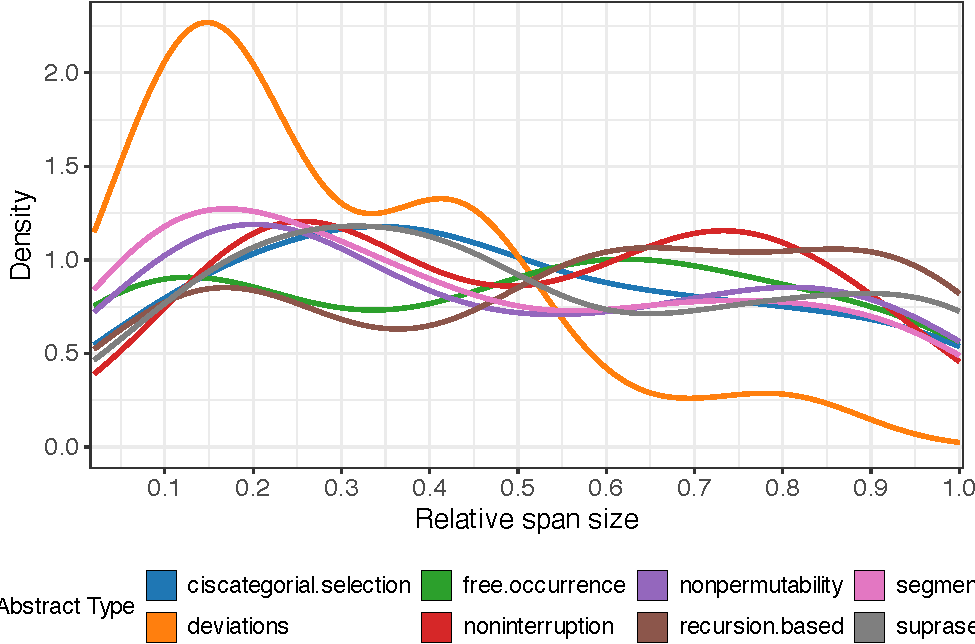
\includegraphics[width=0.9\textwidth,height=\textheight]{02_analyses_chapter17_files/figure-latex/density plot-1} \end{center}

\section{Section 6}\label{section-6}

\subsection{Subsection 6.2}\label{subsection-6.2}

\subsubsection{Correlation plots across abstract
types}\label{correlation-plots-across-abstract-types}

To look at correlations between abstract types of tests, we recode all
variables into binary numeric ones, where 0 indicates absence and 1
presence. We then sum these binary values per abstract type of test for
each language and span. We repeat the same process, but for each
language and left and right edges, respectively.

\begin{Shaded}
\begin{Highlighting}[]
\CommentTok{\# recode the variables to numeric}
\NormalTok{abstract\_type }\OtherTok{\textless{}{-}}\NormalTok{ domains\_verbal\_sub }\SpecialCharTok{\%\textgreater{}\%}
  \FunctionTok{pivot\_wider}\NormalTok{(., }\AttributeTok{names\_from =}\NormalTok{ Abstract\_Type, }\AttributeTok{values\_from =}\NormalTok{ Abstract\_Type) }\SpecialCharTok{\%\textgreater{}\%}
  \FunctionTok{mutate}\NormalTok{(}\FunctionTok{across}\NormalTok{(nonpermutability}\SpecialCharTok{:}\NormalTok{noninterruption, }\SpecialCharTok{\textasciitilde{}} \FunctionTok{if\_else}\NormalTok{(}\FunctionTok{is.na}\NormalTok{(.x), }\DecValTok{0}\NormalTok{, }\DecValTok{1}\NormalTok{)))}
\CommentTok{\# sum overlaps by language and abstract type {-} for the whole span}
\NormalTok{abstract\_type\_span }\OtherTok{\textless{}{-}}\NormalTok{ abstract\_type }\SpecialCharTok{\%\textgreater{}\%}
  \FunctionTok{group\_by}\NormalTok{(Language\_ID, Left\_Edge, Right\_Edge) }\SpecialCharTok{\%\textgreater{}\%}
  \FunctionTok{summarise}\NormalTok{(}
    \AttributeTok{Nonpermut. =} \FunctionTok{sum}\NormalTok{(nonpermutability),}
    \AttributeTok{Noninterrupt. =} \FunctionTok{sum}\NormalTok{(noninterruption),}
    \AttributeTok{Selection. =} \FunctionTok{sum}\NormalTok{(ciscategorial.selection),}
    \AttributeTok{Segmental. =} \FunctionTok{sum}\NormalTok{(segmental),}
    \AttributeTok{Free\_occur. =} \FunctionTok{sum}\NormalTok{(free.occurrence),}
    \AttributeTok{Recursion. =} \FunctionTok{sum}\NormalTok{(recursion.based),}
    \AttributeTok{Supraseg. =} \FunctionTok{sum}\NormalTok{(suprasegmental),}
    \AttributeTok{Deviations. =} \FunctionTok{sum}\NormalTok{(deviations)}
\NormalTok{  ) }\SpecialCharTok{\%\textgreater{}\%}
  \FunctionTok{ungroup}\NormalTok{() }\SpecialCharTok{\%\textgreater{}\%}
  \FunctionTok{select}\NormalTok{(}\SpecialCharTok{{-}}\FunctionTok{c}\NormalTok{(Language\_ID, Left\_Edge, Right\_Edge))}
\end{Highlighting}
\end{Shaded}

\begin{verbatim}
## `summarise()` has grouped output by 'Language_ID', 'Left_Edge'. You can
## override using the `.groups` argument.
\end{verbatim}

\begin{Shaded}
\begin{Highlighting}[]
\FunctionTok{glimpse}\NormalTok{(abstract\_type\_span)}
\end{Highlighting}
\end{Shaded}

\begin{verbatim}
## Rows: 236
## Columns: 8
## $ Nonpermut.    <dbl> 0, 1, 0, 0, 0, 0, 1, 0, 0, 0, 0, 0, 0, 0, 0, 1, 0, 0, 1,~
## $ Noninterrupt. <dbl> 0, 0, 0, 0, 1, 0, 1, 0, 0, 0, 0, 0, 0, 0, 1, 0, 0, 0, 0,~
## $ Selection.    <dbl> 1, 0, 0, 1, 0, 0, 0, 0, 1, 0, 0, 0, 0, 0, 0, 0, 0, 1, 0,~
## $ Segmental.    <dbl> 0, 1, 0, 1, 0, 0, 1, 0, 0, 1, 0, 0, 0, 0, 0, 0, 1, 0, 0,~
## $ Free_occur.   <dbl> 0, 0, 0, 0, 0, 1, 1, 0, 0, 0, 0, 0, 0, 0, 0, 0, 0, 0, 0,~
## $ Recursion.    <dbl> 1, 0, 1, 1, 0, 0, 1, 0, 0, 0, 1, 0, 1, 1, 1, 0, 0, 2, 0,~
## $ Supraseg.     <dbl> 0, 0, 0, 0, 0, 1, 0, 1, 0, 0, 0, 1, 0, 0, 0, 0, 0, 1, 1,~
## $ Deviations.   <dbl> 0, 0, 0, 0, 0, 0, 0, 0, 0, 0, 0, 0, 0, 0, 0, 0, 0, 1, 0,~
\end{verbatim}

\begin{Shaded}
\begin{Highlighting}[]
\CommentTok{\# \# sum overlaps by language and abstract type {-} for the right edge}
\NormalTok{abstract\_type\_right }\OtherTok{\textless{}{-}}\NormalTok{ abstract\_type }\SpecialCharTok{\%\textgreater{}\%}
  \FunctionTok{group\_by}\NormalTok{(Language\_ID, Right\_Edge) }\SpecialCharTok{\%\textgreater{}\%}
  \FunctionTok{summarise}\NormalTok{(}
    \AttributeTok{Nonpermut. =} \FunctionTok{sum}\NormalTok{(nonpermutability),}
    \AttributeTok{Noninterrupt. =} \FunctionTok{sum}\NormalTok{(noninterruption),}
    \AttributeTok{Selection. =} \FunctionTok{sum}\NormalTok{(ciscategorial.selection),}
    \AttributeTok{Segmental. =} \FunctionTok{sum}\NormalTok{(segmental),}
    \AttributeTok{Free\_occur. =} \FunctionTok{sum}\NormalTok{(free.occurrence),}
    \AttributeTok{Recursion. =} \FunctionTok{sum}\NormalTok{(recursion.based),}
    \AttributeTok{Supraseg. =} \FunctionTok{sum}\NormalTok{(suprasegmental),}
    \AttributeTok{Deviations. =} \FunctionTok{sum}\NormalTok{(deviations)}
\NormalTok{  ) }\SpecialCharTok{\%\textgreater{}\%}
  \FunctionTok{ungroup}\NormalTok{() }\SpecialCharTok{\%\textgreater{}\%}
  \FunctionTok{select}\NormalTok{(}\SpecialCharTok{{-}}\FunctionTok{c}\NormalTok{(Language\_ID, Right\_Edge))}
\end{Highlighting}
\end{Shaded}

\begin{verbatim}
## `summarise()` has grouped output by 'Language_ID'. You can override using the
## `.groups` argument.
\end{verbatim}

\begin{Shaded}
\begin{Highlighting}[]
\FunctionTok{glimpse}\NormalTok{(abstract\_type\_right)}
\end{Highlighting}
\end{Shaded}

\begin{verbatim}
## Rows: 139
## Columns: 8
## $ Nonpermut.    <dbl> 2, 0, 0, 0, 0, 0, 0, 0, 1, 1, 0, 0, 0, 0, 0, 0, 0, 0, 1,~
## $ Noninterrupt. <dbl> 1, 0, 0, 0, 0, 1, 0, 0, 0, 0, 0, 2, 0, 0, 0, 0, 0, 0, 1,~
## $ Selection.    <dbl> 0, 0, 1, 0, 1, 0, 1, 1, 0, 0, 0, 1, 0, 0, 0, 0, 0, 0, 2,~
## $ Segmental.    <dbl> 2, 0, 0, 1, 1, 0, 0, 2, 0, 0, 1, 1, 0, 0, 0, 0, 0, 0, 2,~
## $ Free_occur.   <dbl> 1, 0, 0, 0, 0, 0, 1, 1, 0, 0, 0, 1, 0, 0, 0, 0, 0, 0, 1,~
## $ Recursion.    <dbl> 1, 0, 0, 1, 1, 0, 1, 2, 1, 0, 0, 1, 2, 0, 1, 1, 1, 0, 1,~
## $ Supraseg.     <dbl> 0, 1, 0, 0, 0, 0, 1, 2, 2, 2, 0, 2, 0, 1, 0, 0, 0, 0, 1,~
## $ Deviations.   <dbl> 0, 0, 0, 0, 0, 0, 0, 1, 0, 0, 0, 1, 0, 0, 0, 0, 0, 1, 1,~
\end{verbatim}

\begin{Shaded}
\begin{Highlighting}[]
\CommentTok{\# sum overlaps by language and abstract type {-} for the left edge}
\NormalTok{abstract\_type\_left }\OtherTok{\textless{}{-}}\NormalTok{ abstract\_type }\SpecialCharTok{\%\textgreater{}\%}
  \FunctionTok{group\_by}\NormalTok{(Language\_ID, Left\_Edge) }\SpecialCharTok{\%\textgreater{}\%}
  \FunctionTok{summarise}\NormalTok{(}
    \AttributeTok{Nonpermut. =} \FunctionTok{sum}\NormalTok{(nonpermutability),}
    \AttributeTok{Noninterrupt. =} \FunctionTok{sum}\NormalTok{(noninterruption),}
    \AttributeTok{Selection. =} \FunctionTok{sum}\NormalTok{(ciscategorial.selection),}
    \AttributeTok{Segmental. =} \FunctionTok{sum}\NormalTok{(segmental),}
    \AttributeTok{Free\_occur. =} \FunctionTok{sum}\NormalTok{(free.occurrence),}
    \AttributeTok{Recursion. =} \FunctionTok{sum}\NormalTok{(recursion.based),}
    \AttributeTok{Supraseg. =} \FunctionTok{sum}\NormalTok{(suprasegmental),}
    \AttributeTok{Deviations. =} \FunctionTok{sum}\NormalTok{(deviations)}
\NormalTok{  ) }\SpecialCharTok{\%\textgreater{}\%}
  \FunctionTok{ungroup}\NormalTok{() }\SpecialCharTok{\%\textgreater{}\%}
  \FunctionTok{select}\NormalTok{(}\SpecialCharTok{{-}}\FunctionTok{c}\NormalTok{(Language\_ID, Left\_Edge))}
\end{Highlighting}
\end{Shaded}

\begin{verbatim}
## `summarise()` has grouped output by 'Language_ID'. You can override using the
## `.groups` argument.
\end{verbatim}

\begin{Shaded}
\begin{Highlighting}[]
\FunctionTok{glimpse}\NormalTok{(abstract\_type\_left)}
\end{Highlighting}
\end{Shaded}

\begin{verbatim}
## Rows: 96
## Columns: 8
## $ Nonpermut.    <dbl> 0, 1, 1, 0, 0, 0, 1, 1, 0, 0, 2, 0, 0, 0, 0, 3, 0, 0, 2,~
## $ Noninterrupt. <dbl> 0, 1, 1, 0, 0, 1, 0, 1, 0, 0, 1, 0, 0, 0, 0, 2, 0, 0, 1,~
## $ Selection.    <dbl> 1, 1, 1, 0, 0, 0, 0, 2, 0, 0, 1, 1, 0, 1, 0, 0, 2, 0, 1,~
## $ Segmental.    <dbl> 0, 2, 2, 0, 0, 0, 1, 0, 2, 1, 2, 0, 0, 0, 1, 6, 1, 0, 3,~
## $ Free_occur.   <dbl> 0, 1, 1, 0, 0, 0, 0, 1, 0, 1, 2, 0, 0, 0, 0, 1, 1, 0, 1,~
## $ Recursion.    <dbl> 1, 2, 1, 1, 2, 1, 0, 2, 0, 0, 4, 0, 0, 0, 5, 7, 0, 2, 2,~
## $ Supraseg.     <dbl> 0, 1, 1, 1, 0, 0, 0, 6, 0, 2, 2, 0, 0, 2, 1, 3, 1, 0, 0,~
## $ Deviations.   <dbl> 0, 0, 0, 0, 0, 0, 0, 2, 0, 0, 0, 1, 1, 0, 0, 1, 0, 0, 0,~
\end{verbatim}

We then calculate Kendall's tau for each of these data sets and plot the
results as correlation plots.

\begin{Shaded}
\begin{Highlighting}[]
\CommentTok{\# make correlation matrices}
\NormalTok{corr\_span }\OtherTok{\textless{}{-}} \FunctionTok{cor}\NormalTok{(abstract\_type\_span, }\AttributeTok{method =} \StringTok{"kendall"}\NormalTok{)}
\NormalTok{corr\_left }\OtherTok{\textless{}{-}} \FunctionTok{cor}\NormalTok{(abstract\_type\_left, }\AttributeTok{method =} \StringTok{"kendall"}\NormalTok{)}
\NormalTok{corr\_right }\OtherTok{\textless{}{-}} \FunctionTok{cor}\NormalTok{(abstract\_type\_right, }\AttributeTok{method =} \StringTok{"kendall"}\NormalTok{)}

\CommentTok{\# plot correlations}
\NormalTok{plot\_corr\_span }\OtherTok{\textless{}{-}} \FunctionTok{ggcorrplot}\NormalTok{(corr\_span,}
  \AttributeTok{type =} \StringTok{"lower"}\NormalTok{,}
  \AttributeTok{lab =} \ConstantTok{TRUE}\NormalTok{,}
  \AttributeTok{lab\_size =} \DecValTok{4}
\NormalTok{)}
\NormalTok{plot\_corr\_span}
\end{Highlighting}
\end{Shaded}

\begin{center}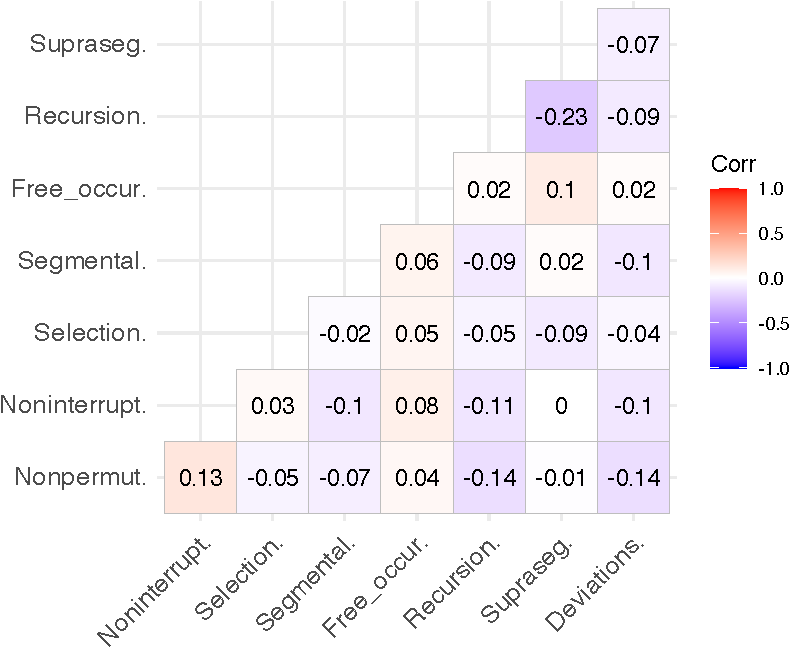
\includegraphics[width=0.9\textwidth,height=\textheight]{02_analyses_chapter17_files/figure-latex/corr plots-1} \end{center}

\begin{Shaded}
\begin{Highlighting}[]
\NormalTok{plot\_corr\_left }\OtherTok{\textless{}{-}} \FunctionTok{ggcorrplot}\NormalTok{(corr\_left,}
  \AttributeTok{type =} \StringTok{"lower"}\NormalTok{,}
  \AttributeTok{lab =} \ConstantTok{TRUE}\NormalTok{,}
  \AttributeTok{lab\_size =} \DecValTok{5}\NormalTok{,}
  \AttributeTok{tl.cex =} \DecValTok{12}
\NormalTok{)}

\NormalTok{plot\_corr\_right }\OtherTok{\textless{}{-}} \FunctionTok{ggcorrplot}\NormalTok{(corr\_right,}
  \AttributeTok{type =} \StringTok{"lower"}\NormalTok{,}
  \AttributeTok{lab =} \ConstantTok{TRUE}\NormalTok{,}
  \AttributeTok{lab\_size =} \DecValTok{5}\NormalTok{,}
  \AttributeTok{tl.cex =} \DecValTok{12}
\NormalTok{)}
\end{Highlighting}
\end{Shaded}

\subsubsection{Correlation tables for cross-language and minimal/maximal
fractures}\label{correlation-tables-for-cross-language-and-minimalmaximal-fractures}

We also want to look at more fine-grained fractures. We thus create new
subsets with the cross-language fractures and the minimal/maximal
fractures, where available. For ciscategorial selection, free
occurrence, recursion based, segmental, and suprasegmental test domains,
we use the minimal/maximal fractures. For deviations from biuniqueness,
non-permutability, and non-interruptability we use the cross-language
fractures.

\begin{Shaded}
\begin{Highlighting}[]
\CommentTok{\# data set for comparing cross{-}language fractures and min{-}max domains}
\NormalTok{cross\_l }\OtherTok{\textless{}{-}}\NormalTok{ domains\_verbal\_sub }\SpecialCharTok{\%\textgreater{}\%}
  \FunctionTok{mutate}\NormalTok{(}\AttributeTok{MinMax\_Fracture =} \FunctionTok{case\_match}\NormalTok{(}
\NormalTok{    MinMax\_Fracture,}
    \StringTok{"minimal"} \SpecialCharTok{\textasciitilde{}} \StringTok{"min"}\NormalTok{,}
    \StringTok{"maximal"} \SpecialCharTok{\textasciitilde{}} \StringTok{"max"}
\NormalTok{  )) }\SpecialCharTok{\%\textgreater{}\%}
  \FunctionTok{mutate}\NormalTok{(}\AttributeTok{abstract\_cross\_l =} \FunctionTok{case\_when}\NormalTok{(}
\NormalTok{    Abstract\_Type }\SpecialCharTok{==} \StringTok{"deviations"} \SpecialCharTok{\textasciitilde{}} \FunctionTok{paste}\NormalTok{(Abstract\_Type, CrossL\_Fracture, }\AttributeTok{sep =} \StringTok{"\_"}\NormalTok{),}
\NormalTok{    Abstract\_Type }\SpecialCharTok{==} \StringTok{"nonpermutability"} \SpecialCharTok{\textasciitilde{}} \FunctionTok{paste}\NormalTok{(Abstract\_Type, CrossL\_Fracture, }\AttributeTok{sep =} \StringTok{"\_"}\NormalTok{),}
\NormalTok{    Abstract\_Type }\SpecialCharTok{==} \StringTok{"noninterruption"} \SpecialCharTok{\textasciitilde{}} \FunctionTok{paste}\NormalTok{(Abstract\_Type, CrossL\_Fracture, }\AttributeTok{sep =} \StringTok{"\_"}\NormalTok{),}
\NormalTok{    Abstract\_Type }\SpecialCharTok{==} \StringTok{"ciscategorial.selection"} \SpecialCharTok{\textasciitilde{}} \FunctionTok{paste}\NormalTok{(Abstract\_Type, MinMax\_Fracture, }\AttributeTok{sep =} \StringTok{"\_"}\NormalTok{),}
\NormalTok{    Abstract\_Type }\SpecialCharTok{==} \StringTok{"free.occurrence"} \SpecialCharTok{\textasciitilde{}} \FunctionTok{paste}\NormalTok{(Abstract\_Type, MinMax\_Fracture, }\AttributeTok{sep =} \StringTok{"\_"}\NormalTok{),}
\NormalTok{    Abstract\_Type }\SpecialCharTok{==} \StringTok{"recursion.based"} \SpecialCharTok{\textasciitilde{}} \FunctionTok{paste}\NormalTok{(Abstract\_Type, MinMax\_Fracture, }\AttributeTok{sep =} \StringTok{"\_"}\NormalTok{),}
\NormalTok{    Abstract\_Type }\SpecialCharTok{==} \StringTok{"segmental"} \SpecialCharTok{\textasciitilde{}} \FunctionTok{paste}\NormalTok{(Abstract\_Type, MinMax\_Fracture, }\AttributeTok{sep =} \StringTok{"\_"}\NormalTok{),}
\NormalTok{    Abstract\_Type }\SpecialCharTok{==} \StringTok{"suprasegmental"} \SpecialCharTok{\textasciitilde{}} \FunctionTok{paste}\NormalTok{(Abstract\_Type, MinMax\_Fracture, }\AttributeTok{sep =} \StringTok{"\_"}\NormalTok{)}
\NormalTok{  )) }\SpecialCharTok{\%\textgreater{}\%}
  \FunctionTok{mutate}\NormalTok{(}
    \AttributeTok{abstract\_cross\_l =} \FunctionTok{str\_remove\_all}\NormalTok{(abstract\_cross\_l, }\StringTok{"\_NA"}\NormalTok{),}
    \AttributeTok{abstract\_cross\_l =} \FunctionTok{if\_else}\NormalTok{(Abstract\_Type }\SpecialCharTok{==} \StringTok{"deviations"}\NormalTok{, Abstract\_Type, abstract\_cross\_l)}
\NormalTok{  ) }\SpecialCharTok{\%\textgreater{}\%}
  \FunctionTok{arrange}\NormalTok{(abstract\_cross\_l) }\SpecialCharTok{\%\textgreater{}\%}
  \FunctionTok{pivot\_wider}\NormalTok{(., }\AttributeTok{names\_from =}\NormalTok{ abstract\_cross\_l, }\AttributeTok{values\_from =}\NormalTok{ abstract\_cross\_l) }\SpecialCharTok{\%\textgreater{}\%}
  \FunctionTok{mutate}\NormalTok{(}\FunctionTok{across}\NormalTok{(ciscategorial.selection}\SpecialCharTok{:}\NormalTok{suprasegmental\_min, }\SpecialCharTok{\textasciitilde{}} \FunctionTok{if\_else}\NormalTok{(}\FunctionTok{is.na}\NormalTok{(.x), }\DecValTok{0}\NormalTok{, }\DecValTok{1}\NormalTok{)))}
\end{Highlighting}
\end{Shaded}

We look at correlations between minimal and maximal domains and
cross-language fractures, respectively. We do this first for the whole
span and then for the right and left edge. Since there are many test
pairs and we are only interested in correlations that are at least
moderate, we summarize the results in tables omitting values between
-0.2 and 0.2.

\begin{Shaded}
\begin{Highlighting}[]
\CommentTok{\# make data set for correlations using whole span}
\NormalTok{cross\_l\_span }\OtherTok{\textless{}{-}}\NormalTok{ cross\_l }\SpecialCharTok{\%\textgreater{}\%}
  \FunctionTok{group\_by}\NormalTok{(Language\_ID, Left\_Edge, Right\_Edge) }\SpecialCharTok{\%\textgreater{}\%}
  \FunctionTok{summarise}\NormalTok{(}
    \AttributeTok{Noninterrupt\_simpl =} \FunctionTok{sum}\NormalTok{(noninterruption\_simplex),}
    \AttributeTok{Noninterrupt\_compl =} \FunctionTok{sum}\NormalTok{(noninterruption\_complex),}
    \AttributeTok{Noninterrupt\_multipos =} \FunctionTok{sum}\NormalTok{(noninterruption\_multipositional),}
    \AttributeTok{Nonpermut\_rigid =} \FunctionTok{sum}\NormalTok{(nonpermutability\_rigid),}
    \AttributeTok{Nonpermut\_scopal =} \FunctionTok{sum}\NormalTok{(nonpermutability\_scopal),}
    \AttributeTok{Selection\_min =} \FunctionTok{sum}\NormalTok{(ciscategorial.selection\_min),}
    \AttributeTok{Selection\_max =} \FunctionTok{sum}\NormalTok{(ciscategorial.selection\_max),}
    \AttributeTok{Recursion\_min =} \FunctionTok{sum}\NormalTok{(recursion.based\_min),}
    \AttributeTok{Recursion\_max =} \FunctionTok{sum}\NormalTok{(recursion.based\_max),}
    \AttributeTok{FreeOccur\_min =} \FunctionTok{sum}\NormalTok{(free.occurrence\_min),}
    \AttributeTok{FreeOccur\_max =} \FunctionTok{sum}\NormalTok{(free.occurrence\_max),}
    \AttributeTok{Deviations =} \FunctionTok{sum}\NormalTok{(deviations),}
    \AttributeTok{Segmental\_min =} \FunctionTok{sum}\NormalTok{(segmental\_min),}
    \AttributeTok{Segmental\_max =} \FunctionTok{sum}\NormalTok{(segmental\_max),}
    \AttributeTok{Supraseg\_min =} \FunctionTok{sum}\NormalTok{(suprasegmental\_min),}
    \AttributeTok{Supraseg\_max =} \FunctionTok{sum}\NormalTok{(suprasegmental\_min)}
\NormalTok{  ) }\SpecialCharTok{\%\textgreater{}\%}
  \FunctionTok{ungroup}\NormalTok{()}
\end{Highlighting}
\end{Shaded}

\begin{verbatim}
## `summarise()` has grouped output by 'Language_ID', 'Left_Edge'. You can
## override using the `.groups` argument.
\end{verbatim}

\begin{Shaded}
\begin{Highlighting}[]
\FunctionTok{glimpse}\NormalTok{(cross\_l\_span)}
\end{Highlighting}
\end{Shaded}

\begin{verbatim}
## Rows: 236
## Columns: 19
## $ Language_ID           <chr> "arao1248", "arao1248", "arao1248", "arao1248", ~
## $ Left_Edge             <dbl> 1, 4, 4, 4, 4, 4, 6, 6, 6, 6, 2, 2, 3, 3, 6, 13,~
## $ Right_Edge            <dbl> 17, 6, 14, 15, 16, 17, 6, 11, 13, 14, 29, 31, 20~
## $ Noninterrupt_simpl    <dbl> 0, 0, 0, 0, 0, 0, 1, 0, 0, 0, 0, 0, 0, 0, 0, 0, ~
## $ Noninterrupt_compl    <dbl> 0, 0, 0, 0, 1, 0, 0, 0, 0, 0, 0, 0, 0, 0, 1, 0, ~
## $ Noninterrupt_multipos <dbl> 0, 0, 0, 0, 0, 0, 0, 0, 0, 0, 0, 0, 0, 0, 0, 0, ~
## $ Nonpermut_rigid       <dbl> 0, 0, 0, 0, 0, 0, 1, 0, 0, 0, 0, 0, 0, 0, 0, 0, ~
## $ Nonpermut_scopal      <dbl> 0, 1, 0, 0, 0, 0, 0, 0, 0, 0, 0, 0, 0, 0, 0, 1, ~
## $ Selection_min         <dbl> 0, 0, 0, 0, 0, 0, 0, 0, 1, 0, 0, 0, 0, 0, 0, 0, ~
## $ Selection_max         <dbl> 1, 0, 0, 1, 0, 0, 0, 0, 0, 0, 0, 0, 0, 0, 0, 0, ~
## $ Recursion_min         <dbl> 0, 0, 1, 0, 0, 0, 1, 0, 0, 0, 0, 0, 1, 0, 1, 0, ~
## $ Recursion_max         <dbl> 1, 0, 0, 1, 0, 0, 0, 0, 0, 0, 1, 0, 0, 1, 0, 0, ~
## $ FreeOccur_min         <dbl> 0, 0, 0, 0, 0, 0, 1, 0, 0, 0, 0, 0, 0, 0, 0, 0, ~
## $ FreeOccur_max         <dbl> 0, 0, 0, 0, 0, 1, 0, 0, 0, 0, 0, 0, 0, 0, 0, 0, ~
## $ Deviations            <dbl> 0, 0, 0, 0, 0, 0, 0, 0, 0, 0, 0, 0, 0, 0, 0, 0, ~
## $ Segmental_min         <dbl> 0, 0, 0, 0, 0, 0, 1, 0, 0, 0, 0, 0, 0, 0, 0, 0, ~
## $ Segmental_max         <dbl> 0, 0, 0, 0, 0, 0, 0, 0, 0, 1, 0, 0, 0, 0, 0, 0, ~
## $ Supraseg_min          <dbl> 0, 0, 0, 0, 0, 0, 0, 1, 0, 0, 0, 0, 0, 0, 0, 0, ~
## $ Supraseg_max          <dbl> 0, 0, 0, 0, 0, 0, 0, 1, 0, 0, 0, 0, 0, 0, 0, 0, ~
\end{verbatim}

\begin{Shaded}
\begin{Highlighting}[]
\CommentTok{\# minimal domains and cross{-}language fractures}
\NormalTok{cross\_l\_min }\OtherTok{\textless{}{-}} \FunctionTok{select}\NormalTok{(cross\_l\_span, }\SpecialCharTok{{-}}\FunctionTok{ends\_with}\NormalTok{(}\StringTok{"\_max"}\NormalTok{), }\SpecialCharTok{{-}}\FunctionTok{c}\NormalTok{(Language\_ID}\SpecialCharTok{:}\NormalTok{Right\_Edge))}
\CommentTok{\# maximal domains and cross{-}language fractures}
\NormalTok{cross\_l\_max }\OtherTok{\textless{}{-}} \FunctionTok{select}\NormalTok{(cross\_l\_span, }\SpecialCharTok{{-}}\FunctionTok{ends\_with}\NormalTok{(}\StringTok{"\_min"}\NormalTok{), }\SpecialCharTok{{-}}\FunctionTok{c}\NormalTok{(Language\_ID}\SpecialCharTok{:}\NormalTok{Right\_Edge))}
\CommentTok{\# correlation matrices}
\NormalTok{corr\_cross\_l\_min }\OtherTok{\textless{}{-}} \FunctionTok{cor}\NormalTok{(cross\_l\_min, }\AttributeTok{method =} \StringTok{"kendall"}\NormalTok{)}
\NormalTok{corr\_cross\_l\_max }\OtherTok{\textless{}{-}} \FunctionTok{cor}\NormalTok{(cross\_l\_max, }\AttributeTok{method =} \StringTok{"kendall"}\NormalTok{)}
\end{Highlighting}
\end{Shaded}

\begin{Shaded}
\begin{Highlighting}[]
\CommentTok{\# same but with edge convergences instead of whole span}
\CommentTok{\# left edge:}
\NormalTok{cross\_l\_left }\OtherTok{\textless{}{-}}\NormalTok{ cross\_l }\SpecialCharTok{\%\textgreater{}\%}
  \FunctionTok{group\_by}\NormalTok{(Language\_ID, Left\_Edge) }\SpecialCharTok{\%\textgreater{}\%}
  \FunctionTok{summarise}\NormalTok{(}
    \AttributeTok{Noninterrupt\_simpl =} \FunctionTok{sum}\NormalTok{(noninterruption\_simplex),}
    \AttributeTok{Noninterrupt\_compl =} \FunctionTok{sum}\NormalTok{(noninterruption\_complex),}
    \AttributeTok{Noninterrupt\_multipos =} \FunctionTok{sum}\NormalTok{(noninterruption\_multipositional),}
    \AttributeTok{Nonpermut\_rigid =} \FunctionTok{sum}\NormalTok{(nonpermutability\_rigid),}
    \AttributeTok{Nonpermut\_scopal =} \FunctionTok{sum}\NormalTok{(nonpermutability\_scopal),}
    \AttributeTok{Selection\_min =} \FunctionTok{sum}\NormalTok{(ciscategorial.selection\_min),}
    \AttributeTok{Selection\_max =} \FunctionTok{sum}\NormalTok{(ciscategorial.selection\_max),}
    \AttributeTok{Recursion\_min =} \FunctionTok{sum}\NormalTok{(recursion.based\_min),}
    \AttributeTok{Recursion\_max =} \FunctionTok{sum}\NormalTok{(recursion.based\_max),}
    \AttributeTok{FreeOccur\_min =} \FunctionTok{sum}\NormalTok{(free.occurrence\_min),}
    \AttributeTok{FreeOccur\_max =} \FunctionTok{sum}\NormalTok{(free.occurrence\_max),}
    \AttributeTok{Deviations =} \FunctionTok{sum}\NormalTok{(deviations),}
    \AttributeTok{Segmental\_min =} \FunctionTok{sum}\NormalTok{(segmental\_min),}
    \AttributeTok{Segmental\_max =} \FunctionTok{sum}\NormalTok{(segmental\_max),}
    \AttributeTok{Supraseg\_min =} \FunctionTok{sum}\NormalTok{(suprasegmental\_min),}
    \AttributeTok{Supraseg\_max =} \FunctionTok{sum}\NormalTok{(suprasegmental\_min)}
\NormalTok{  ) }\SpecialCharTok{\%\textgreater{}\%}
  \FunctionTok{ungroup}\NormalTok{()}

\CommentTok{\# right edge:}
\NormalTok{cross\_l\_right }\OtherTok{\textless{}{-}}\NormalTok{ cross\_l }\SpecialCharTok{\%\textgreater{}\%}
  \FunctionTok{group\_by}\NormalTok{(Language\_ID, Right\_Edge) }\SpecialCharTok{\%\textgreater{}\%}
  \FunctionTok{summarise}\NormalTok{(}
    \AttributeTok{Noninterrupt\_simpl =} \FunctionTok{sum}\NormalTok{(noninterruption\_simplex),}
    \AttributeTok{Noninterrupt\_compl =} \FunctionTok{sum}\NormalTok{(noninterruption\_complex),}
    \AttributeTok{Noninterrupt\_multipos =} \FunctionTok{sum}\NormalTok{(noninterruption\_multipositional),}
    \AttributeTok{Nonpermut\_rigid =} \FunctionTok{sum}\NormalTok{(nonpermutability\_rigid),}
    \AttributeTok{Nonpermut\_scopal =} \FunctionTok{sum}\NormalTok{(nonpermutability\_scopal),}
    \AttributeTok{Selection\_min =} \FunctionTok{sum}\NormalTok{(ciscategorial.selection\_min),}
    \AttributeTok{Selection\_max =} \FunctionTok{sum}\NormalTok{(ciscategorial.selection\_max),}
    \AttributeTok{Recursion\_min =} \FunctionTok{sum}\NormalTok{(recursion.based\_min),}
    \AttributeTok{Recursion\_max =} \FunctionTok{sum}\NormalTok{(recursion.based\_max),}
    \AttributeTok{FreeOccur\_min =} \FunctionTok{sum}\NormalTok{(free.occurrence\_min),}
    \AttributeTok{FreeOccur\_max =} \FunctionTok{sum}\NormalTok{(free.occurrence\_max),}
    \AttributeTok{Deviations =} \FunctionTok{sum}\NormalTok{(deviations),}
    \AttributeTok{Segmental\_min =} \FunctionTok{sum}\NormalTok{(segmental\_min),}
    \AttributeTok{Segmental\_max =} \FunctionTok{sum}\NormalTok{(segmental\_max),}
    \AttributeTok{Supraseg\_min =} \FunctionTok{sum}\NormalTok{(suprasegmental\_min),}
    \AttributeTok{Supraseg\_max =} \FunctionTok{sum}\NormalTok{(suprasegmental\_min)}
\NormalTok{  ) }\SpecialCharTok{\%\textgreater{}\%}
  \FunctionTok{ungroup}\NormalTok{()}

\CommentTok{\# minimal domains and cross{-}language fractures {-} left edges}
\NormalTok{cross\_l\_min\_left }\OtherTok{\textless{}{-}} \FunctionTok{select}\NormalTok{(cross\_l\_left, }\SpecialCharTok{{-}}\FunctionTok{ends\_with}\NormalTok{(}\StringTok{"\_max"}\NormalTok{), }\SpecialCharTok{{-}}\FunctionTok{c}\NormalTok{(Language\_ID}\SpecialCharTok{:}\NormalTok{Left\_Edge))}
\CommentTok{\# maximal domains and cross{-}language fractures}
\NormalTok{cross\_l\_max\_left }\OtherTok{\textless{}{-}} \FunctionTok{select}\NormalTok{(cross\_l\_left, }\SpecialCharTok{{-}}\FunctionTok{ends\_with}\NormalTok{(}\StringTok{"\_min"}\NormalTok{), }\SpecialCharTok{{-}}\FunctionTok{c}\NormalTok{(Language\_ID}\SpecialCharTok{:}\NormalTok{Left\_Edge))}

\CommentTok{\# minimal domains and cross{-}language fractures {-} right edges}
\NormalTok{cross\_l\_min\_right }\OtherTok{\textless{}{-}} \FunctionTok{select}\NormalTok{(cross\_l\_right, }\SpecialCharTok{{-}}\FunctionTok{ends\_with}\NormalTok{(}\StringTok{"\_max"}\NormalTok{), }\SpecialCharTok{{-}}\FunctionTok{c}\NormalTok{(Language\_ID}\SpecialCharTok{:}\NormalTok{Right\_Edge))}
\CommentTok{\# maximal domains and cross{-}language fractures}
\NormalTok{cross\_l\_max\_right }\OtherTok{\textless{}{-}} \FunctionTok{select}\NormalTok{(cross\_l\_right, }\SpecialCharTok{{-}}\FunctionTok{ends\_with}\NormalTok{(}\StringTok{"\_min"}\NormalTok{), }\SpecialCharTok{{-}}\FunctionTok{c}\NormalTok{(Language\_ID}\SpecialCharTok{:}\NormalTok{Right\_Edge))}
\end{Highlighting}
\end{Shaded}

To create the correlation tables efficiently, we set up a custom
function.

\begin{Shaded}
\begin{Highlighting}[]
\CommentTok{\# set up function to create correlation dataframes}
\NormalTok{corr\_to\_df }\OtherTok{\textless{}{-}} \ControlFlowTok{function}\NormalTok{(x, y, z, a, b, c) \{}
\NormalTok{  df1 }\OtherTok{\textless{}{-}} \FunctionTok{cor}\NormalTok{(x, }\AttributeTok{method =} \StringTok{"kendall"}\NormalTok{) }\SpecialCharTok{\%\textgreater{}\%}
    \FunctionTok{as.data.frame}\NormalTok{() }\SpecialCharTok{\%\textgreater{}\%}
    \FunctionTok{rownames\_to\_column}\NormalTok{(., }\AttributeTok{var =} \StringTok{"Test1"}\NormalTok{) }\SpecialCharTok{\%\textgreater{}\%}
    \FunctionTok{pivot\_longer}\NormalTok{(}\SpecialCharTok{{-}}\NormalTok{Test1, }\AttributeTok{names\_to =} \StringTok{"Test2"}\NormalTok{, }\AttributeTok{values\_to =} \FunctionTok{paste0}\NormalTok{(y, }\StringTok{"."}\NormalTok{, z))}
\NormalTok{  df2 }\OtherTok{\textless{}{-}} \FunctionTok{cor}\NormalTok{(a, }\AttributeTok{method =} \StringTok{"kendall"}\NormalTok{) }\SpecialCharTok{\%\textgreater{}\%}
    \FunctionTok{as.data.frame}\NormalTok{() }\SpecialCharTok{\%\textgreater{}\%}
    \FunctionTok{rownames\_to\_column}\NormalTok{(., }\AttributeTok{var =} \StringTok{"Test1"}\NormalTok{) }\SpecialCharTok{\%\textgreater{}\%}
    \FunctionTok{pivot\_longer}\NormalTok{(}\SpecialCharTok{{-}}\NormalTok{Test1, }\AttributeTok{names\_to =} \StringTok{"Test2"}\NormalTok{, }\AttributeTok{values\_to =} \FunctionTok{paste0}\NormalTok{(b, }\StringTok{"."}\NormalTok{, c)) }\SpecialCharTok{\%\textgreater{}\%}
    \FunctionTok{select}\NormalTok{(}\SpecialCharTok{{-}}\FunctionTok{c}\NormalTok{(Test1, Test2))}
  \CommentTok{\# full correlation df}
\NormalTok{  corr\_full }\OtherTok{\textless{}{-}} \FunctionTok{bind\_cols}\NormalTok{(df1, df2) }\SpecialCharTok{\%\textgreater{}\%}
    \FunctionTok{distinct}\NormalTok{(}\FunctionTok{across}\NormalTok{(}\FunctionTok{starts\_with}\NormalTok{(}\StringTok{"M"}\NormalTok{)), }\AttributeTok{.keep\_all =} \ConstantTok{TRUE}\NormalTok{) }\SpecialCharTok{\%\textgreater{}\%}
    \FunctionTok{filter}\NormalTok{(Test1 }\SpecialCharTok{!=}\NormalTok{ Test2) }\SpecialCharTok{\%\textgreater{}\%}
    \FunctionTok{kable}\NormalTok{(}
      \AttributeTok{booktabs =} \ConstantTok{TRUE}\NormalTok{, }\AttributeTok{linesep =} \StringTok{""}\NormalTok{,}
      \AttributeTok{align =} \StringTok{"llrr"}
\NormalTok{    )}
  \CommentTok{\# excluding weak correlations and highlighting cells with higher correlations; exporting table to latex}
\NormalTok{  corr\_higher }\OtherTok{\textless{}{-}} \FunctionTok{bind\_cols}\NormalTok{(df1, df2) }\SpecialCharTok{\%\textgreater{}\%}
    \FunctionTok{distinct}\NormalTok{(}\FunctionTok{across}\NormalTok{(}\FunctionTok{starts\_with}\NormalTok{(}\StringTok{"M"}\NormalTok{)), }\AttributeTok{.keep\_all =} \ConstantTok{TRUE}\NormalTok{) }\SpecialCharTok{\%\textgreater{}\%}
    \FunctionTok{filter}\NormalTok{(Test1 }\SpecialCharTok{!=}\NormalTok{ Test2) }\SpecialCharTok{\%\textgreater{}\%}
    \FunctionTok{mutate}\NormalTok{(}\FunctionTok{across}\NormalTok{(}\FunctionTok{starts\_with}\NormalTok{(}\StringTok{"M"}\NormalTok{), }\SpecialCharTok{\textasciitilde{}} \FunctionTok{round}\NormalTok{(.x, }\DecValTok{2}\NormalTok{))) }\SpecialCharTok{\%\textgreater{}\%}
    \FunctionTok{mutate}\NormalTok{(}\FunctionTok{across}\NormalTok{(}\FunctionTok{starts\_with}\NormalTok{(}\StringTok{"M"}\NormalTok{), }\SpecialCharTok{\textasciitilde{}} \FunctionTok{case\_when}\NormalTok{(}
\NormalTok{      .x }\SpecialCharTok{\textgreater{}} \FloatTok{0.3} \SpecialCharTok{\textasciitilde{}} \FunctionTok{paste0}\NormalTok{(}\StringTok{"}\SpecialCharTok{\textbackslash{}\textbackslash{}}\StringTok{cellcolor\{red!45\}"}\NormalTok{, .x),}
      \FunctionTok{between}\NormalTok{(.x, }\FloatTok{0.2}\NormalTok{, }\FloatTok{0.3}\NormalTok{) }\SpecialCharTok{\textasciitilde{}} \FunctionTok{paste0}\NormalTok{(}\StringTok{"}\SpecialCharTok{\textbackslash{}\textbackslash{}}\StringTok{cellcolor\{red!25\}"}\NormalTok{, .x),}
\NormalTok{      .x }\SpecialCharTok{\textless{}} \SpecialCharTok{{-}}\FloatTok{0.3} \SpecialCharTok{\textasciitilde{}} \FunctionTok{paste0}\NormalTok{(}\StringTok{"}\SpecialCharTok{\textbackslash{}\textbackslash{}}\StringTok{cellcolor\{blue!45\}"}\NormalTok{, .x),}
      \FunctionTok{between}\NormalTok{(.x, }\FloatTok{0.2}\NormalTok{, }\FloatTok{0.3}\NormalTok{) }\SpecialCharTok{\textasciitilde{}} \FunctionTok{paste0}\NormalTok{(}\StringTok{"}\SpecialCharTok{\textbackslash{}\textbackslash{}}\StringTok{cellcolor\{blue!25\}"}\NormalTok{, .x),}
      \AttributeTok{.default =} \FunctionTok{paste}\NormalTok{(.x)}
\NormalTok{    ))) }\SpecialCharTok{\%\textgreater{}\%}
    \FunctionTok{mutate}\NormalTok{(}\FunctionTok{across}\NormalTok{(}\FunctionTok{starts\_with}\NormalTok{(}\StringTok{"Test"}\NormalTok{), }\SpecialCharTok{\textasciitilde{}} \FunctionTok{str\_replace\_all}\NormalTok{(.x, }\StringTok{"\_"}\NormalTok{, }\StringTok{"."}\NormalTok{))) }\SpecialCharTok{\%\textgreater{}\%}
    \FunctionTok{filter}\NormalTok{(}\FunctionTok{if\_any}\NormalTok{(}\FunctionTok{starts\_with}\NormalTok{(}\StringTok{"M"}\NormalTok{), }\SpecialCharTok{\textasciitilde{}} \FunctionTok{str\_detect}\NormalTok{(., }\StringTok{"cellcolor"}\NormalTok{))) }\SpecialCharTok{\%\textgreater{}\%}
    \FunctionTok{kable}\NormalTok{(}
      \AttributeTok{booktabs =} \ConstantTok{TRUE}\NormalTok{, }\AttributeTok{format =} \StringTok{"latex"}\NormalTok{, }\AttributeTok{escape =} \ConstantTok{FALSE}\NormalTok{, }\AttributeTok{linesep =} \StringTok{""}\NormalTok{,}
      \AttributeTok{align =} \StringTok{"llrr"}
\NormalTok{    ) }\SpecialCharTok{\%\textgreater{}\%}
    \FunctionTok{kable\_styling}\NormalTok{()}
  \CommentTok{\# return full df and latex table}
  \FunctionTok{return}\NormalTok{(}\FunctionTok{list}\NormalTok{(corr\_full, corr\_higher))}
\NormalTok{\}}
\end{Highlighting}
\end{Shaded}

We apply the function to each subset and display the full correlation
tables. The highlighted tables are exported for inclusion in the
chapter.

\begin{Shaded}
\begin{Highlighting}[]
\CommentTok{\# cross{-}language + min/max {-} whole span}
\NormalTok{corr\_cross\_l\_span }\OtherTok{\textless{}{-}} \FunctionTok{corr\_to\_df}\NormalTok{(cross\_l\_min, }\StringTok{"Min"}\NormalTok{, }\StringTok{"Span"}\NormalTok{, cross\_l\_max, }\StringTok{"Max"}\NormalTok{, }\StringTok{"Span"}\NormalTok{)}
\NormalTok{corr\_cross\_l\_span[[}\DecValTok{1}\NormalTok{]]}
\end{Highlighting}
\end{Shaded}

\begin{longtable}[]{@{}llrr@{}}
\toprule\noalign{}
Test1 & Test2 & Min.Span & Max.Span \\
\midrule\noalign{}
\endhead
\bottomrule\noalign{}
\endlastfoot
Noninterrupt\_simpl & Noninterrupt\_compl & -0.0350877 & -0.0350877 \\
Noninterrupt\_simpl & Noninterrupt\_multipos & -0.0245959 &
-0.0245959 \\
Noninterrupt\_simpl & Nonpermut\_rigid & 0.1431491 & 0.1431491 \\
Noninterrupt\_simpl & Nonpermut\_scopal & -0.0327498 & -0.0327498 \\
Noninterrupt\_simpl & Selection\_min & -0.0470398 & 0.0383744 \\
Noninterrupt\_simpl & Recursion\_min & 0.0910499 & -0.0681671 \\
Noninterrupt\_simpl & FreeOccur\_min & 0.0306309 & 0.2027476 \\
Noninterrupt\_simpl & Deviations & 0.0024339 & 0.0024339 \\
Noninterrupt\_simpl & Segmental\_min & 0.0860252 & -0.0596055 \\
Noninterrupt\_simpl & Supraseg\_min & 0.0085362 & 0.0085362 \\
Noninterrupt\_compl & Nonpermut\_rigid & -0.0488008 & -0.0488008 \\
Noninterrupt\_compl & Selection\_min & -0.0470398 & -0.0521891 \\
Noninterrupt\_compl & Recursion\_min & 0.0140833 & -0.0681671 \\
Noninterrupt\_compl & FreeOccur\_min & -0.0554274 & -0.0554274 \\
Noninterrupt\_compl & Deviations & -0.0681498 & -0.0681498 \\
Noninterrupt\_compl & Segmental\_min & 0.0109136 & -0.0596055 \\
Noninterrupt\_compl & Supraseg\_min & 0.0828325 & 0.0828325 \\
Noninterrupt\_multipos & Nonpermut\_rigid & -0.0342086 & -0.0342086 \\
Noninterrupt\_multipos & Nonpermut\_scopal & -0.0229571 & -0.0229571 \\
Noninterrupt\_multipos & Selection\_min & 0.2449508 & -0.0365838 \\
Noninterrupt\_multipos & Recursion\_min & -0.0440803 & -0.0477841 \\
Noninterrupt\_multipos & FreeOccur\_min & -0.0388537 & 0.0817974 \\
Noninterrupt\_multipos & Deviations & -0.0477720 & -0.0477720 \\
Noninterrupt\_multipos & Segmental\_min & -0.0450017 & -0.0417825 \\
Noninterrupt\_multipos & Supraseg\_min & -0.0460968 & -0.0460968 \\
Nonpermut\_rigid & Nonpermut\_scopal & -0.0455492 & -0.0455492 \\
Nonpermut\_rigid & Selection\_min & 0.0081001 & -0.0054084 \\
Nonpermut\_rigid & Recursion\_min & 0.0267238 & -0.0948084 \\
Nonpermut\_rigid & FreeOccur\_min & 0.0505817 & 0.0505817 \\
Nonpermut\_rigid & Deviations & -0.0947844 & -0.0947844 \\
Nonpermut\_rigid & Segmental\_min & 0.0280959 & -0.0829007 \\
Nonpermut\_rigid & Supraseg\_min & -0.0363498 & -0.0363498 \\
Nonpermut\_scopal & Selection\_min & -0.0439055 & -0.0487117 \\
Nonpermut\_scopal & Recursion\_min & -0.0586934 & -0.0636251 \\
Nonpermut\_scopal & FreeOccur\_min & -0.0517343 & 0.1318640 \\
Nonpermut\_scopal & Deviations & -0.0636090 & -0.0636090 \\
Nonpermut\_scopal & Segmental\_min & -0.0599204 & -0.0556340 \\
Nonpermut\_scopal & Supraseg\_min & -0.0613785 & -0.0613785 \\
Selection\_min & Recursion\_min & 0.0336211 & 0.0468614 \\
Selection\_min & FreeOccur\_min & 0.1234739 & 0.0380306 \\
Selection\_min & Deviations & 0.0230740 & -0.0519604 \\
Selection\_min & Segmental\_min & 0.0290165 & -0.0886566 \\
Selection\_min & Supraseg\_min & 0.0825896 & 0.0061962 \\
Recursion\_min & FreeOccur\_min & 0.2590134 & -0.0137639 \\
Recursion\_min & Deviations & 0.0087240 & -0.1323989 \\
Recursion\_min & Segmental\_min & 0.1131364 & -0.0259420 \\
Recursion\_min & Supraseg\_min & -0.0736586 & -0.0872182 \\
FreeOccur\_min & Deviations & 0.0910615 & -0.0607077 \\
FreeOccur\_min & Segmental\_min & 0.2982587 & -0.0418979 \\
FreeOccur\_min & Supraseg\_min & 0.0937864 & -0.0050468 \\
Deviations & Segmental\_min & 0.0488071 & -0.1157700 \\
Deviations & Supraseg\_min & 0.0391242 & 0.0391242 \\
Segmental\_min & Supraseg\_min & 0.1863994 & -0.0164050 \\
\end{longtable}

\begin{Shaded}
\begin{Highlighting}[]
\CommentTok{\# cross{-}language + minimal {-} left/right}
\NormalTok{corr\_cross\_l\_min }\OtherTok{\textless{}{-}} \FunctionTok{corr\_to\_df}\NormalTok{(cross\_l\_min\_left, }\StringTok{"Min"}\NormalTok{, }\StringTok{"Left"}\NormalTok{, cross\_l\_min\_right, }\StringTok{"Min"}\NormalTok{, }\StringTok{"Right"}\NormalTok{)}
\NormalTok{corr\_cross\_l\_min[[}\DecValTok{1}\NormalTok{]]}
\end{Highlighting}
\end{Shaded}

\begin{longtable}[]{@{}llrr@{}}
\toprule\noalign{}
Test1 & Test2 & Min.Left & Min.Right \\
\midrule\noalign{}
\endhead
\bottomrule\noalign{}
\endlastfoot
Noninterrupt\_simpl & Noninterrupt\_compl & 0.0586075 & 0.2041985 \\
Noninterrupt\_simpl & Noninterrupt\_multipos & 0.1538093 & -0.0425375 \\
Noninterrupt\_simpl & Nonpermut\_rigid & 0.3817291 & 0.1131670 \\
Noninterrupt\_simpl & Nonpermut\_scopal & 0.0734833 & 0.0843454 \\
Noninterrupt\_simpl & Selection\_min & 0.2571236 & -0.0827024 \\
Noninterrupt\_simpl & Recursion\_min & 0.0884481 & 0.2159912 \\
Noninterrupt\_simpl & FreeOccur\_min & -0.0396129 & -0.0039560 \\
Noninterrupt\_simpl & Deviations & 0.2272164 & 0.0413788 \\
Noninterrupt\_simpl & Segmental\_min & 0.2919756 & 0.0507138 \\
Noninterrupt\_simpl & Supraseg\_min & 0.1680648 & -0.0320786 \\
Noninterrupt\_compl & Noninterrupt\_multipos & -0.0628695 & 0.1422349 \\
Noninterrupt\_compl & Nonpermut\_rigid & 0.1194933 & -0.0859497 \\
Noninterrupt\_compl & Nonpermut\_scopal & 0.2053565 & -0.0569077 \\
Noninterrupt\_compl & Selection\_min & 0.0981295 & -0.0827024 \\
Noninterrupt\_compl & Recursion\_min & 0.4573045 & 0.0534044 \\
Noninterrupt\_compl & FreeOccur\_min & 0.1340079 & -0.0039560 \\
Noninterrupt\_compl & Deviations & 0.0763835 & 0.0540223 \\
Noninterrupt\_compl & Segmental\_min & 0.2138178 & 0.0642767 \\
Noninterrupt\_compl & Supraseg\_min & 0.2277638 & 0.1277312 \\
Noninterrupt\_multipos & Nonpermut\_rigid & 0.0729153 & 0.0788268 \\
Noninterrupt\_multipos & Nonpermut\_scopal & 0.1420172 & 0.1571412 \\
Noninterrupt\_multipos & Selection\_min & 0.3882387 & 0.2283690 \\
Noninterrupt\_multipos & Recursion\_min & -0.0947373 & 0.0371990 \\
Noninterrupt\_multipos & FreeOccur\_min & -0.1035780 & 0.0606219 \\
Noninterrupt\_multipos & Deviations & 0.0236155 & 0.0464363 \\
Noninterrupt\_multipos & Segmental\_min & 0.0442955 & 0.0542194 \\
Noninterrupt\_multipos & Supraseg\_min & 0.0158837 & 0.0333135 \\
Nonpermut\_rigid & Nonpermut\_scopal & 0.2577841 & 0.2379919 \\
Nonpermut\_rigid & Selection\_min & 0.1995048 & 0.1147347 \\
Nonpermut\_rigid & Recursion\_min & 0.1786094 & 0.0904180 \\
Nonpermut\_rigid & FreeOccur\_min & 0.0414455 & 0.1484730 \\
Nonpermut\_rigid & Deviations & 0.0140816 & 0.1419272 \\
Nonpermut\_rigid & Segmental\_min & 0.1165267 & -0.0230173 \\
Nonpermut\_rigid & Supraseg\_min & 0.3614843 & 0.0223279 \\
Nonpermut\_scopal & Selection\_min & 0.1200822 & 0.0322425 \\
Nonpermut\_scopal & Recursion\_min & 0.0910146 & -0.0151667 \\
Nonpermut\_scopal & FreeOccur\_min & -0.0387557 & 0.0084261 \\
Nonpermut\_scopal & Deviations & -0.0640026 & -0.1028252 \\
Nonpermut\_scopal & Segmental\_min & 0.0650839 & -0.0163285 \\
Nonpermut\_scopal & Supraseg\_min & 0.1719241 & -0.1043535 \\
Selection\_min & Recursion\_min & 0.1302715 & 0.0408683 \\
Selection\_min & FreeOccur\_min & 0.2556631 & 0.3643023 \\
Selection\_min & Deviations & 0.1775783 & 0.0982878 \\
Selection\_min & Segmental\_min & 0.1876479 & 0.0378763 \\
Selection\_min & Supraseg\_min & 0.2406169 & 0.1060675 \\
Recursion\_min & FreeOccur\_min & 0.3116368 & 0.2927496 \\
Recursion\_min & Deviations & 0.1809762 & 0.0636153 \\
Recursion\_min & Segmental\_min & 0.3039147 & 0.1155138 \\
Recursion\_min & Supraseg\_min & 0.2436265 & -0.0043524 \\
FreeOccur\_min & Deviations & 0.2231660 & 0.2946544 \\
FreeOccur\_min & Segmental\_min & 0.4292868 & 0.4054280 \\
FreeOccur\_min & Supraseg\_min & 0.3697661 & 0.2289099 \\
Deviations & Segmental\_min & 0.3843538 & 0.1275054 \\
Deviations & Supraseg\_min & 0.2306674 & 0.1510526 \\
Segmental\_min & Supraseg\_min & 0.3617206 & 0.2278026 \\
\end{longtable}

\begin{Shaded}
\begin{Highlighting}[]
\CommentTok{\# cross{-}language + maximal {-} left/right}
\NormalTok{corr\_cross\_l\_max }\OtherTok{\textless{}{-}} \FunctionTok{corr\_to\_df}\NormalTok{(cross\_l\_max\_left, }\StringTok{"Max"}\NormalTok{, }\StringTok{"Left"}\NormalTok{, cross\_l\_max\_right, }\StringTok{"Max"}\NormalTok{, }\StringTok{"Right"}\NormalTok{)}
\NormalTok{corr\_cross\_l\_max[[}\DecValTok{1}\NormalTok{]]}
\end{Highlighting}
\end{Shaded}

\begin{longtable}[]{@{}llrr@{}}
\toprule\noalign{}
Test1 & Test2 & Max.Left & Max.Right \\
\midrule\noalign{}
\endhead
\bottomrule\noalign{}
\endlastfoot
Noninterrupt\_simpl & Noninterrupt\_compl & 0.0586075 & 0.2041985 \\
Noninterrupt\_simpl & Noninterrupt\_multipos & 0.1538093 & -0.0425375 \\
Noninterrupt\_simpl & Nonpermut\_rigid & 0.3817291 & 0.1131670 \\
Noninterrupt\_simpl & Nonpermut\_scopal & 0.0734833 & 0.0843454 \\
Noninterrupt\_simpl & Selection\_max & 0.1882274 & 0.0020349 \\
Noninterrupt\_simpl & Recursion\_max & -0.0520398 & 0.0467851 \\
Noninterrupt\_simpl & FreeOccur\_max & 0.2574835 & 0.2774557 \\
Noninterrupt\_simpl & Deviations & 0.2272164 & 0.0413788 \\
Noninterrupt\_simpl & Segmental\_max & 0.2722157 & -0.0079399 \\
Noninterrupt\_simpl & Supraseg\_max & 0.1680648 & -0.0320786 \\
Noninterrupt\_compl & Noninterrupt\_multipos & -0.0628695 & 0.1422349 \\
Noninterrupt\_compl & Nonpermut\_rigid & 0.1194933 & -0.0859497 \\
Noninterrupt\_compl & Nonpermut\_scopal & 0.2053565 & -0.0569077 \\
Noninterrupt\_compl & Selection\_max & 0.0575922 & 0.0020349 \\
Noninterrupt\_compl & Recursion\_max & 0.1677723 & -0.1076057 \\
Noninterrupt\_compl & FreeOccur\_max & 0.2286017 & 0.0929342 \\
Noninterrupt\_compl & Deviations & 0.0763835 & 0.0540223 \\
Noninterrupt\_compl & Segmental\_max & 0.1244123 & -0.0079399 \\
Noninterrupt\_compl & Supraseg\_max & 0.2277638 & 0.1277312 \\
Noninterrupt\_multipos & Nonpermut\_rigid & 0.0729153 & 0.0788268 \\
Noninterrupt\_multipos & Nonpermut\_scopal & 0.1420172 & 0.1571412 \\
Noninterrupt\_multipos & Selection\_max & 0.1763842 & -0.0642551 \\
Noninterrupt\_multipos & Recursion\_max & -0.1166327 & -0.0749530 \\
Noninterrupt\_multipos & FreeOccur\_max & 0.0272574 & 0.0647335 \\
Noninterrupt\_multipos & Deviations & 0.0236155 & 0.0464363 \\
Noninterrupt\_multipos & Segmental\_max & 0.1642564 & -0.0714714 \\
Noninterrupt\_multipos & Supraseg\_max & 0.0158837 & 0.0333135 \\
Nonpermut\_rigid & Nonpermut\_scopal & 0.2577841 & 0.2379919 \\
Nonpermut\_rigid & Selection\_max & 0.0737923 & 0.0117103 \\
Nonpermut\_rigid & Recursion\_max & -0.0565064 & -0.0355571 \\
Nonpermut\_rigid & FreeOccur\_max & 0.5241642 & 0.0096045 \\
Nonpermut\_rigid & Deviations & 0.0140816 & 0.1419272 \\
Nonpermut\_rigid & Segmental\_max & 0.1826726 & -0.0733522 \\
Nonpermut\_rigid & Supraseg\_max & 0.3614843 & 0.0223279 \\
Nonpermut\_scopal & Selection\_max & -0.0251447 & -0.0859620 \\
Nonpermut\_scopal & Recursion\_max & 0.0326811 & -0.1002739 \\
Nonpermut\_scopal & FreeOccur\_max & 0.2629103 & 0.1111662 \\
Nonpermut\_scopal & Deviations & -0.0640026 & -0.1028252 \\
Nonpermut\_scopal & Segmental\_max & 0.1522914 & -0.0956161 \\
Nonpermut\_scopal & Supraseg\_max & 0.1719241 & -0.1043535 \\
Selection\_max & Recursion\_max & 0.0839477 & 0.0773226 \\
Selection\_max & FreeOccur\_max & 0.2489805 & 0.1321240 \\
Selection\_max & Deviations & 0.0845809 & 0.1147964 \\
Selection\_max & Segmental\_max & -0.0293431 & 0.0468888 \\
Selection\_max & Supraseg\_max & 0.0464228 & 0.1716444 \\
Recursion\_max & FreeOccur\_max & 0.0243731 & 0.0160968 \\
Recursion\_max & Deviations & 0.0755752 & -0.0961583 \\
Recursion\_max & Segmental\_max & 0.0442958 & 0.0524054 \\
Recursion\_max & Supraseg\_max & 0.0970535 & -0.0428956 \\
FreeOccur\_max & Deviations & -0.0311684 & -0.0073009 \\
FreeOccur\_max & Segmental\_max & 0.0614584 & 0.1146591 \\
FreeOccur\_max & Supraseg\_max & 0.2781544 & -0.0498077 \\
Deviations & Segmental\_max & 0.1460861 & -0.0838708 \\
Deviations & Supraseg\_max & 0.2306674 & 0.1510526 \\
Segmental\_max & Supraseg\_max & 0.2952724 & -0.0235193 \\
\end{longtable}

\subsection{Subsection 6.3}\label{subsection-6.3}

\subsubsection{Density plot of relative convergences across span and
edges}\label{density-plot-of-relative-convergences-across-span-and-edges}

In order to assess if there are overall tendencies for some domains to
converge than others, we explore the density distributions of span and
edge convergences pooled across languages of the sample. We do this by
calculating the the convergences across the span, and on the right and
left edge and displaying the densities of these distributions.

\begin{Shaded}
\begin{Highlighting}[]
\CommentTok{\# calculate right and left edge convergences}
\NormalTok{domains\_verbal }\OtherTok{\textless{}{-}}\NormalTok{ domains\_verbal }\SpecialCharTok{\%\textgreater{}\%}
  \FunctionTok{group\_by}\NormalTok{(Language\_ID, Left\_Edge) }\SpecialCharTok{\%\textgreater{}\%}
  \FunctionTok{mutate}\NormalTok{(}\AttributeTok{Convergence\_Left =} \FunctionTok{n}\NormalTok{()) }\SpecialCharTok{\%\textgreater{}\%}
  \FunctionTok{group\_by}\NormalTok{(Language\_ID, Right\_Edge) }\SpecialCharTok{\%\textgreater{}\%}
  \FunctionTok{mutate}\NormalTok{(}\AttributeTok{Convergence\_Right =} \FunctionTok{n}\NormalTok{()) }\SpecialCharTok{\%\textgreater{}\%}
  \FunctionTok{ungroup}\NormalTok{() }\SpecialCharTok{\%\textgreater{}\%}
  \FunctionTok{mutate}\NormalTok{(}\AttributeTok{Relative\_Convergence\_Left =} \FunctionTok{round}\NormalTok{(Convergence\_Left }\SpecialCharTok{/}\NormalTok{ Tests\_Total, }\DecValTok{2}\NormalTok{), }\AttributeTok{Relative\_Convergence\_Right =} \FunctionTok{round}\NormalTok{(Convergence\_Right }\SpecialCharTok{/}\NormalTok{ Tests\_Total, }\DecValTok{2}\NormalTok{))}
\FunctionTok{glimpse}\NormalTok{(domains\_verbal)}
\end{Highlighting}
\end{Shaded}

\begin{verbatim}
## Rows: 388
## Columns: 26
## $ Serial_Order               <dbl> 366, 239, 224, 25, 40, 44, 178, 180, 182, 1~
## $ Language_Name              <fct> South Bolivian Quechua, Chorote, Hup, Ayaut~
## $ Language_ID                <chr> "sout2991", "iyoj1235", "hupd1244", "ayau12~
## $ Domain_ID                  <fct> "sout2991_v_nonpermutability_minimal_chi.(1~
## $ Domain_Type                <fct> morphosyntactic, indeterminate, morphosynta~
## $ Abstract_Type              <fct> nonpermutability, free.occurrence, recursio~
## $ CrossL_Fracture            <fct> NA, NA, NA, NA, vowel-consonant.dissimilati~
## $ MinMax_Fracture            <fct> minimal, minimal, NA, minimal, minimal, min~
## $ Lspecific_Fracture         <fct> "chi.(13).and.chi.(18).not.one.morpheme", N~
## $ Left_Edge                  <dbl> 12, 16, 6, 19, 19, 19, 17, 17, 17, 17, 17, ~
## $ Right_Edge                 <dbl> 12, 16, 6, 19, 19, 19, 17, 17, 17, 17, 17, ~
## $ Convergence                <dbl> 1, 1, 1, 3, 3, 3, 6, 6, 6, 6, 6, 6, 1, 1, 1~
## $ Relative_Convergence       <dbl> 0.05, 0.04, 0.07, 0.10, 0.10, 0.10, 0.22, 0~
## $ Size                       <dbl> 1, 1, 1, 1, 1, 1, 1, 1, 1, 1, 1, 1, 1, 2, 2~
## $ Relative_Size              <dbl> 0.02, 0.03, 0.03, 0.03, 0.03, 0.03, 0.03, 0~
## $ Largest                    <dbl> 42, 37, 32, 30, 30, 30, 29, 29, 29, 29, 29,~
## $ Position_Total             <dbl> 42, 46, 32, 31, 31, 31, 29, 29, 29, 29, 29,~
## $ Tests_Total                <dbl> 20, 28, 15, 30, 30, 30, 27, 27, 27, 27, 27,~
## $ Planar_ID                  <fct> sout2991_verbal, iyoj1235_verbal, hupd1244_~
## $ PW_Pattern                 <fct> morphosyntactic, indeterminate, morphosynta~
## $ Test_Labels                <fct> Non-permut., NA, Subspan Rep. Base, Min Fre~
## $ Short_Name                 <chr> "SB Quechua", "Chorote", "Hup", "Ayautla Ma~
## $ Convergence_Left           <int> 16, 6, 4, 4, 4, 4, 8, 8, 8, 8, 8, 8, 3, 1, ~
## $ Convergence_Right          <int> 1, 4, 1, 9, 9, 9, 8, 8, 8, 8, 8, 8, 2, 4, 1~
## $ Relative_Convergence_Left  <dbl> 0.80, 0.21, 0.27, 0.13, 0.13, 0.13, 0.30, 0~
## $ Relative_Convergence_Right <dbl> 0.05, 0.14, 0.07, 0.30, 0.30, 0.30, 0.30, 0~
\end{verbatim}

\begin{Shaded}
\begin{Highlighting}[]
\CommentTok{\# data set for plotting density}
\NormalTok{domains\_verbal\_density }\OtherTok{\textless{}{-}}\NormalTok{ domains\_verbal }\SpecialCharTok{\%\textgreater{}\%}
  \FunctionTok{rename}\NormalTok{(}
    \AttributeTok{Span =}\NormalTok{ Relative\_Convergence,}
    \AttributeTok{Left =}\NormalTok{ Relative\_Convergence\_Left,}
    \AttributeTok{Right =}\NormalTok{ Relative\_Convergence\_Right}
\NormalTok{  ) }\SpecialCharTok{\%\textgreater{}\%}
  \FunctionTok{distinct}\NormalTok{(Language\_ID, Span, Right, Left) }\SpecialCharTok{\%\textgreater{}\%}
  \FunctionTok{pivot\_longer}\NormalTok{(}\SpecialCharTok{{-}}\NormalTok{Language\_ID, }\AttributeTok{names\_to =} \StringTok{"Convergence\_Type"}\NormalTok{, }\AttributeTok{values\_to =} \StringTok{"Relative\_Convergence"}\NormalTok{) }\SpecialCharTok{\%\textgreater{}\%}
  \FunctionTok{mutate}\NormalTok{(}\AttributeTok{Convergence\_Type =} \FunctionTok{factor}\NormalTok{(Convergence\_Type, }\AttributeTok{levels =} \FunctionTok{c}\NormalTok{(}\StringTok{"Span"}\NormalTok{, }\StringTok{"Left"}\NormalTok{, }\StringTok{"Right"}\NormalTok{)))}

\CommentTok{\# density plot across all languages}
\NormalTok{plot\_density\_all }\OtherTok{\textless{}{-}} \FunctionTok{ggplot}\NormalTok{(}\AttributeTok{data =}\NormalTok{ domains\_verbal\_density, }\FunctionTok{aes}\NormalTok{(}\AttributeTok{x =}\NormalTok{ Relative\_Convergence, }\AttributeTok{group =}\NormalTok{ Convergence\_Type, }\AttributeTok{fill =}\NormalTok{ Convergence\_Type)) }\SpecialCharTok{+}
  \FunctionTok{geom\_density}\NormalTok{(}\AttributeTok{alpha =} \FloatTok{0.6}\NormalTok{) }\SpecialCharTok{+}
  \FunctionTok{scale\_fill\_d3}\NormalTok{(}\AttributeTok{name =} \StringTok{"Type of Convergence"}\NormalTok{) }\SpecialCharTok{+}
  \CommentTok{\# guides(fill = guide\_legend(override.aes = list(alpha = 1, linewidth = 0))) +}
  \FunctionTok{labs}\NormalTok{(}\AttributeTok{x =} \StringTok{"Relative convergence"}\NormalTok{, }\AttributeTok{y =} \StringTok{"Density"}\NormalTok{, ) }\SpecialCharTok{+}
  \FunctionTok{scale\_x\_continuous}\NormalTok{(}\AttributeTok{expand =} \FunctionTok{c}\NormalTok{(}\FloatTok{0.005}\NormalTok{, }\FloatTok{0.005}\NormalTok{), }\AttributeTok{breaks =} \FunctionTok{seq}\NormalTok{(}\DecValTok{0}\NormalTok{, }\DecValTok{1}\NormalTok{, }\FloatTok{0.2}\NormalTok{)) }\SpecialCharTok{+}
  \FunctionTok{theme\_bw}\NormalTok{() }\SpecialCharTok{+}
  \FunctionTok{theme}\NormalTok{(}
    \AttributeTok{legend.position =} \FunctionTok{c}\NormalTok{(}\FloatTok{0.85}\NormalTok{, }\FloatTok{0.85}\NormalTok{),}
    \CommentTok{\# legend.key.size = unit(1, "lines"),}
    \AttributeTok{legend.text =} \FunctionTok{element\_text}\NormalTok{(}\AttributeTok{size =} \DecValTok{11}\NormalTok{),}
    \AttributeTok{axis.text =} \FunctionTok{element\_text}\NormalTok{(}\AttributeTok{size =} \DecValTok{12}\NormalTok{),}
    \AttributeTok{axis.title =} \FunctionTok{element\_text}\NormalTok{(}\AttributeTok{size =} \DecValTok{13}\NormalTok{),}
    \AttributeTok{strip.text.x =} \FunctionTok{element\_text}\NormalTok{(}\AttributeTok{size =} \DecValTok{11}\NormalTok{)}
\NormalTok{  )}
\NormalTok{plot\_density\_all}
\end{Highlighting}
\end{Shaded}

\begin{center}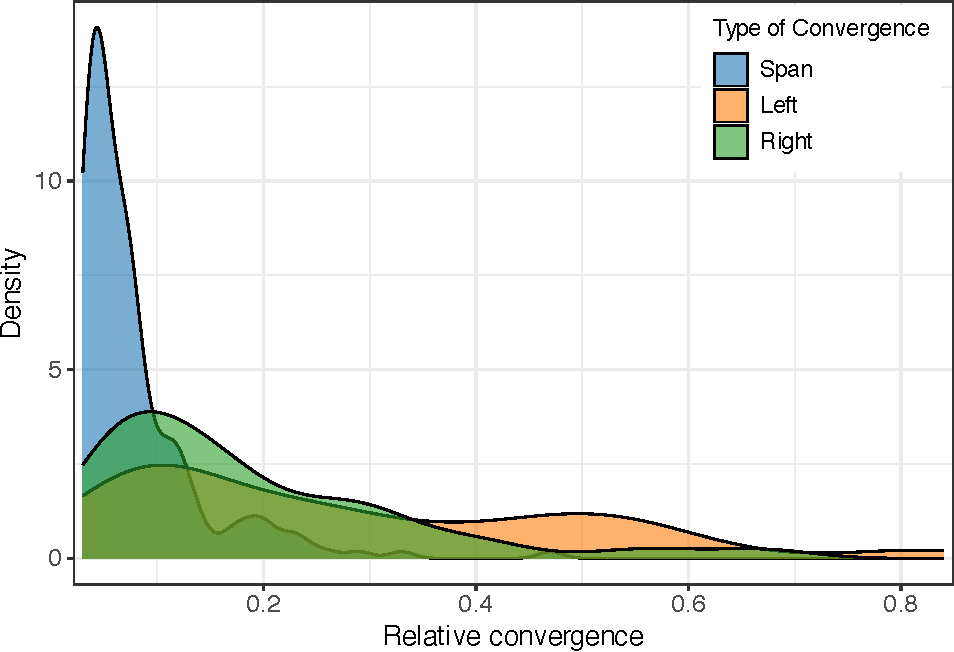
\includegraphics[width=0.9\textwidth,height=\textheight]{02_analyses_chapter17_files/figure-latex/dens rconv-1} \end{center}

\subsubsection{Density plots of relative span convergence per abstract
type}\label{density-plots-of-relative-span-convergence-per-abstract-type}

We do the same, but separating the tests by abstract type. We exclude
types with fewer than 5 data points, because these are not informative.

\begin{Shaded}
\begin{Highlighting}[]
\CommentTok{\# facet density plot of relative convergence per abstract type}
\NormalTok{plot\_dens\_conv\_atype }\OtherTok{\textless{}{-}} \FunctionTok{ggplot}\NormalTok{(}\FunctionTok{aes}\NormalTok{(}\AttributeTok{x =}\NormalTok{ Relative\_Convergence, }\AttributeTok{group =}\NormalTok{ Abstract\_Type), }\AttributeTok{data =}\NormalTok{ domains\_verbal\_sub) }\SpecialCharTok{+}
  \FunctionTok{geom\_density}\NormalTok{(}\FunctionTok{aes}\NormalTok{(}\AttributeTok{fill =}\NormalTok{ Abstract\_Type)) }\SpecialCharTok{+}
  \FunctionTok{scale\_fill\_d3}\NormalTok{(}\AttributeTok{guide =} \StringTok{"none"}\NormalTok{) }\SpecialCharTok{+}
  \FunctionTok{facet\_wrap}\NormalTok{(}\SpecialCharTok{\textasciitilde{}}\NormalTok{Abstract\_Type, }\AttributeTok{scales =} \StringTok{"free\_x"}\NormalTok{) }\SpecialCharTok{+}
  \FunctionTok{labs}\NormalTok{(}\AttributeTok{x =} \StringTok{"Relative convergence"}\NormalTok{, }\AttributeTok{y =} \StringTok{"Density"}\NormalTok{, ) }\SpecialCharTok{+}
  \FunctionTok{scale\_x\_continuous}\NormalTok{(}\AttributeTok{expand =} \FunctionTok{c}\NormalTok{(}\FloatTok{0.008}\NormalTok{, }\DecValTok{0}\NormalTok{), }\AttributeTok{breaks =} \FunctionTok{seq}\NormalTok{(}\DecValTok{0}\NormalTok{, }\DecValTok{5}\NormalTok{, }\FloatTok{0.1}\NormalTok{), }\AttributeTok{limits =} \FunctionTok{c}\NormalTok{(}\DecValTok{0}\NormalTok{, }\FloatTok{0.5}\NormalTok{)) }\SpecialCharTok{+}
  \FunctionTok{scale\_y\_continuous}\NormalTok{(}\AttributeTok{breaks =} \FunctionTok{seq}\NormalTok{(}\DecValTok{0}\NormalTok{, }\DecValTok{14}\NormalTok{, }\DecValTok{2}\NormalTok{), }\AttributeTok{limits =} \FunctionTok{c}\NormalTok{(}\DecValTok{0}\NormalTok{, }\DecValTok{14}\NormalTok{)) }\SpecialCharTok{+}
  \FunctionTok{theme\_bw}\NormalTok{() }\SpecialCharTok{+}
  \FunctionTok{theme}\NormalTok{(}
    \AttributeTok{legend.position =} \StringTok{"bottom"}\NormalTok{,}
    \AttributeTok{legend.key.size =} \FunctionTok{unit}\NormalTok{(}\DecValTok{1}\NormalTok{, }\StringTok{"lines"}\NormalTok{),}
    \AttributeTok{legend.text =} \FunctionTok{element\_text}\NormalTok{(}\AttributeTok{size =} \DecValTok{11}\NormalTok{),}
    \AttributeTok{axis.text =} \FunctionTok{element\_text}\NormalTok{(}\AttributeTok{size =} \DecValTok{12}\NormalTok{),}
    \AttributeTok{axis.title =} \FunctionTok{element\_text}\NormalTok{(}\AttributeTok{size =} \DecValTok{13}\NormalTok{),}
    \AttributeTok{strip.text.x =} \FunctionTok{element\_text}\NormalTok{(}\AttributeTok{size =} \DecValTok{11}\NormalTok{),}
    \AttributeTok{panel.spacing =} \FunctionTok{unit}\NormalTok{(}\FloatTok{1.3}\NormalTok{, }\StringTok{"lines"}\NormalTok{),}
    \AttributeTok{strip.clip =} \StringTok{"off"}
\NormalTok{  )}
\NormalTok{plot\_dens\_conv\_atype}
\end{Highlighting}
\end{Shaded}

\begin{center}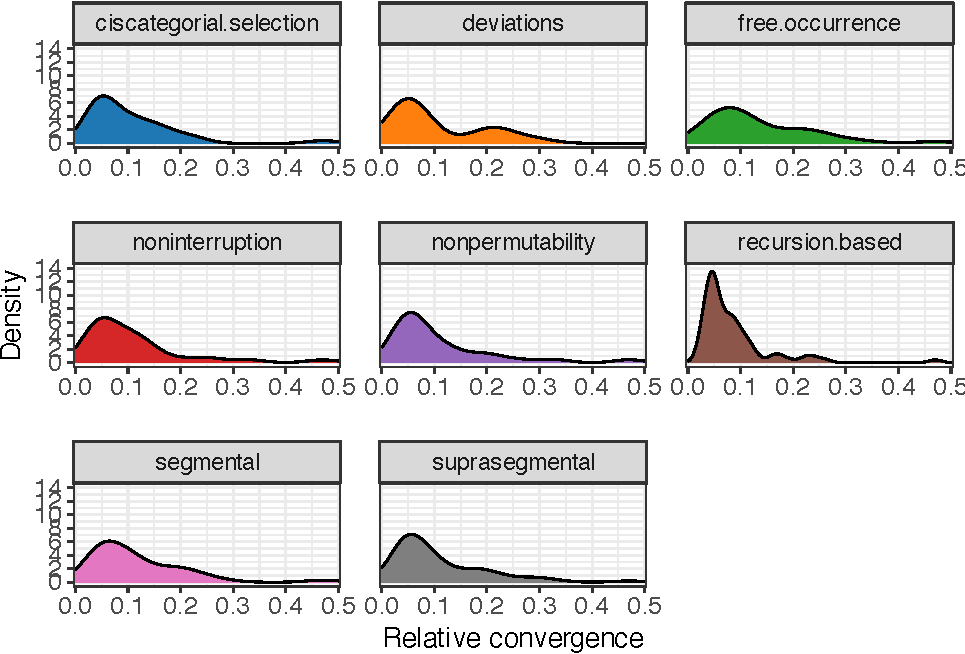
\includegraphics[width=0.9\textwidth,height=\textheight]{02_analyses_chapter17_files/figure-latex/dens at-1} \end{center}

\subsubsection{Density plots of relative span convergence per prosodic
word
domain}\label{density-plots-of-relative-span-convergence-per-prosodic-word-domain}

Next, we look at the distributions by type of prosodic word domain. We
exclude types with fewer than 5 data points, because these are not
informative.

\begin{Shaded}
\begin{Highlighting}[]
\CommentTok{\# exclude categories with few data points}
\NormalTok{keep\_pw }\OtherTok{\textless{}{-}}\NormalTok{ domains\_verbal\_sub }\SpecialCharTok{\%\textgreater{}\%}
  \FunctionTok{count}\NormalTok{(PW\_Pattern) }\SpecialCharTok{\%\textgreater{}\%}
  \FunctionTok{filter}\NormalTok{(n }\SpecialCharTok{\textgreater{}} \DecValTok{5}\NormalTok{) }\SpecialCharTok{\%\textgreater{}\%}
  \FunctionTok{droplevels}\NormalTok{() }\SpecialCharTok{\%\textgreater{}\%}
  \FunctionTok{pull}\NormalTok{(PW\_Pattern)}

\NormalTok{domains\_verbal\_sub\_pw }\OtherTok{\textless{}{-}}\NormalTok{ domains\_verbal\_sub }\SpecialCharTok{\%\textgreater{}\%}
  \FunctionTok{filter}\NormalTok{(PW\_Pattern }\SpecialCharTok{\%in\%}\NormalTok{ keep\_pw) }\SpecialCharTok{\%\textgreater{}\%}
  \FunctionTok{droplevels}\NormalTok{()}

\CommentTok{\# make plot}
\NormalTok{plot\_dens\_conv\_pw }\OtherTok{\textless{}{-}} \FunctionTok{ggplot}\NormalTok{(}\FunctionTok{aes}\NormalTok{(}\AttributeTok{x =}\NormalTok{ Relative\_Convergence, }\AttributeTok{group =}\NormalTok{ PW\_Pattern), }\AttributeTok{data =}\NormalTok{ domains\_verbal\_sub\_pw) }\SpecialCharTok{+}
  \FunctionTok{geom\_density}\NormalTok{(}\FunctionTok{aes}\NormalTok{(}\AttributeTok{fill =}\NormalTok{ PW\_Pattern)) }\SpecialCharTok{+}
  \FunctionTok{scale\_fill\_d3}\NormalTok{(}\AttributeTok{guide =} \StringTok{"none"}\NormalTok{) }\SpecialCharTok{+}
  \FunctionTok{facet\_wrap}\NormalTok{(}\SpecialCharTok{\textasciitilde{}}\NormalTok{PW\_Pattern, }\AttributeTok{scales =} \StringTok{"free\_x"}\NormalTok{, }\AttributeTok{ncol =} \DecValTok{3}\NormalTok{) }\SpecialCharTok{+}
  \FunctionTok{labs}\NormalTok{(}\AttributeTok{x =} \StringTok{"Relative convergence"}\NormalTok{, }\AttributeTok{y =} \StringTok{"Density"}\NormalTok{, ) }\SpecialCharTok{+}
  \FunctionTok{scale\_x\_continuous}\NormalTok{(}\AttributeTok{expand =} \FunctionTok{c}\NormalTok{(}\FloatTok{0.008}\NormalTok{, }\DecValTok{0}\NormalTok{), }\AttributeTok{breaks =} \FunctionTok{seq}\NormalTok{(}\DecValTok{0}\NormalTok{, }\DecValTok{5}\NormalTok{, }\FloatTok{0.1}\NormalTok{), }\AttributeTok{limits =} \FunctionTok{c}\NormalTok{(}\DecValTok{0}\NormalTok{, }\FloatTok{0.5}\NormalTok{)) }\SpecialCharTok{+}
  \FunctionTok{scale\_y\_continuous}\NormalTok{(}\AttributeTok{breaks =} \FunctionTok{seq}\NormalTok{(}\DecValTok{0}\NormalTok{, }\DecValTok{11}\NormalTok{, }\DecValTok{2}\NormalTok{), }\AttributeTok{limits =} \FunctionTok{c}\NormalTok{(}\DecValTok{0}\NormalTok{, }\DecValTok{11}\NormalTok{)) }\SpecialCharTok{+}
  \FunctionTok{theme\_bw}\NormalTok{() }\SpecialCharTok{+}
  \FunctionTok{theme}\NormalTok{(}
    \AttributeTok{legend.position =} \StringTok{"bottom"}\NormalTok{,}
    \AttributeTok{legend.key.size =} \FunctionTok{unit}\NormalTok{(}\DecValTok{1}\NormalTok{, }\StringTok{"lines"}\NormalTok{),}
    \AttributeTok{legend.text =} \FunctionTok{element\_text}\NormalTok{(}\AttributeTok{size =} \DecValTok{11}\NormalTok{),}
    \AttributeTok{axis.text =} \FunctionTok{element\_text}\NormalTok{(}\AttributeTok{size =} \DecValTok{12}\NormalTok{),}
    \AttributeTok{axis.title =} \FunctionTok{element\_text}\NormalTok{(}\AttributeTok{size =} \DecValTok{13}\NormalTok{),}
    \AttributeTok{strip.text.x =} \FunctionTok{element\_text}\NormalTok{(}\AttributeTok{size =} \DecValTok{11}\NormalTok{),}
    \AttributeTok{panel.spacing =} \FunctionTok{unit}\NormalTok{(}\FloatTok{1.3}\NormalTok{, }\StringTok{"lines"}\NormalTok{),}
    \AttributeTok{strip.clip =} \StringTok{"off"}
\NormalTok{  )}
\NormalTok{plot\_dens\_conv\_pw}
\end{Highlighting}
\end{Shaded}

\begin{center}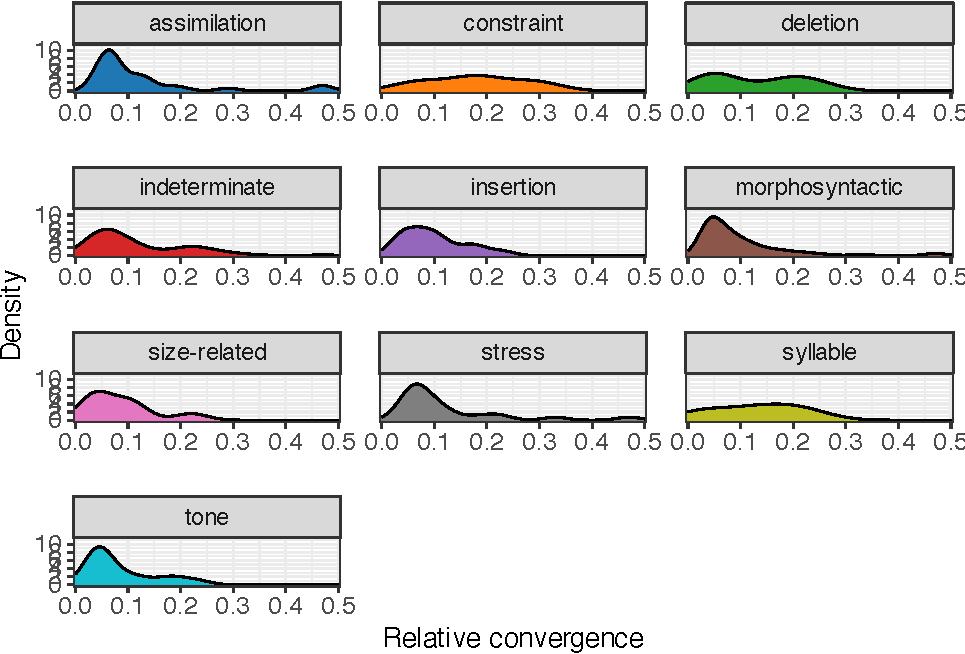
\includegraphics[width=0.9\textwidth,height=\textheight]{02_analyses_chapter17_files/figure-latex/dens pw-1} \end{center}

\subsubsection{Density plots of relative span convergence across
cross-language
fractures}\label{density-plots-of-relative-span-convergence-across-cross-language-fractures}

Lastly, we do the same but look at cross-linguistic fractures with more
than 10 tokens each.

\begin{Shaded}
\begin{Highlighting}[]
\CommentTok{\# take subset with fractures that have more than 10 tokens; exclude NA}
\NormalTok{keep\_clf }\OtherTok{\textless{}{-}}\NormalTok{ domains\_verbal }\SpecialCharTok{\%\textgreater{}\%}
  \FunctionTok{filter}\NormalTok{(}\SpecialCharTok{!}\FunctionTok{is.na}\NormalTok{(CrossL\_Fracture)) }\SpecialCharTok{\%\textgreater{}\%}
  \FunctionTok{count}\NormalTok{(CrossL\_Fracture) }\SpecialCharTok{\%\textgreater{}\%}
  \FunctionTok{filter}\NormalTok{(n }\SpecialCharTok{\textgreater{}} \DecValTok{10}\NormalTok{) }\SpecialCharTok{\%\textgreater{}\%}
  \FunctionTok{droplevels}\NormalTok{() }\SpecialCharTok{\%\textgreater{}\%}
  \FunctionTok{pull}\NormalTok{(CrossL\_Fracture)}
\NormalTok{domains\_verbal\_clf }\OtherTok{\textless{}{-}}\NormalTok{ domains\_verbal }\SpecialCharTok{\%\textgreater{}\%}
  \FunctionTok{filter}\NormalTok{(CrossL\_Fracture }\SpecialCharTok{\%in\%}\NormalTok{ keep\_clf) }\SpecialCharTok{\%\textgreater{}\%}
  \FunctionTok{droplevels}\NormalTok{()}

\CommentTok{\# make plot}
\NormalTok{plot\_dens\_conv\_clf }\OtherTok{\textless{}{-}} \FunctionTok{ggplot}\NormalTok{(}\FunctionTok{aes}\NormalTok{(}\AttributeTok{x =}\NormalTok{ Relative\_Convergence, }\AttributeTok{group =}\NormalTok{ CrossL\_Fracture), }\AttributeTok{data =}\NormalTok{ domains\_verbal\_clf) }\SpecialCharTok{+}
  \FunctionTok{geom\_density}\NormalTok{(}\FunctionTok{aes}\NormalTok{(}\AttributeTok{fill =}\NormalTok{ CrossL\_Fracture)) }\SpecialCharTok{+}
  \FunctionTok{scale\_fill\_d3}\NormalTok{(}\AttributeTok{guide =} \StringTok{"none"}\NormalTok{) }\SpecialCharTok{+}
  \FunctionTok{facet\_wrap}\NormalTok{(}\SpecialCharTok{\textasciitilde{}}\NormalTok{CrossL\_Fracture, }\AttributeTok{scales =} \StringTok{"free\_x"}\NormalTok{, }\AttributeTok{ncol =} \DecValTok{3}\NormalTok{) }\SpecialCharTok{+}
  \FunctionTok{labs}\NormalTok{(}\AttributeTok{x =} \StringTok{"Relative convergence"}\NormalTok{, }\AttributeTok{y =} \StringTok{"Density"}\NormalTok{, ) }\SpecialCharTok{+}
  \FunctionTok{scale\_x\_continuous}\NormalTok{(}\AttributeTok{expand =} \FunctionTok{c}\NormalTok{(}\FloatTok{0.008}\NormalTok{, }\DecValTok{0}\NormalTok{), }\AttributeTok{breaks =} \FunctionTok{seq}\NormalTok{(}\DecValTok{0}\NormalTok{, }\DecValTok{5}\NormalTok{, }\FloatTok{0.1}\NormalTok{), }\AttributeTok{limits =} \FunctionTok{c}\NormalTok{(}\DecValTok{0}\NormalTok{, }\FloatTok{0.5}\NormalTok{)) }\SpecialCharTok{+}
  \FunctionTok{scale\_y\_continuous}\NormalTok{(}\AttributeTok{breaks =} \FunctionTok{seq}\NormalTok{(}\DecValTok{0}\NormalTok{, }\DecValTok{11}\NormalTok{, }\DecValTok{2}\NormalTok{), }\AttributeTok{limits =} \FunctionTok{c}\NormalTok{(}\DecValTok{0}\NormalTok{, }\DecValTok{11}\NormalTok{)) }\SpecialCharTok{+}
  \FunctionTok{theme\_bw}\NormalTok{() }\SpecialCharTok{+}
  \FunctionTok{theme}\NormalTok{(}
    \AttributeTok{legend.position =} \StringTok{"bottom"}\NormalTok{,}
    \AttributeTok{legend.key.size =} \FunctionTok{unit}\NormalTok{(}\DecValTok{1}\NormalTok{, }\StringTok{"lines"}\NormalTok{),}
    \AttributeTok{legend.text =} \FunctionTok{element\_text}\NormalTok{(}\AttributeTok{size =} \DecValTok{11}\NormalTok{),}
    \AttributeTok{axis.text =} \FunctionTok{element\_text}\NormalTok{(}\AttributeTok{size =} \DecValTok{12}\NormalTok{),}
    \AttributeTok{axis.title =} \FunctionTok{element\_text}\NormalTok{(}\AttributeTok{size =} \DecValTok{13}\NormalTok{),}
    \AttributeTok{strip.text.x =} \FunctionTok{element\_text}\NormalTok{(}\AttributeTok{size =} \DecValTok{11}\NormalTok{),}
    \AttributeTok{panel.spacing =} \FunctionTok{unit}\NormalTok{(}\FloatTok{1.3}\NormalTok{, }\StringTok{"lines"}\NormalTok{),}
    \AttributeTok{strip.clip =} \StringTok{"off"}
\NormalTok{  )}
\NormalTok{plot\_dens\_conv\_clf}
\end{Highlighting}
\end{Shaded}

\begin{center}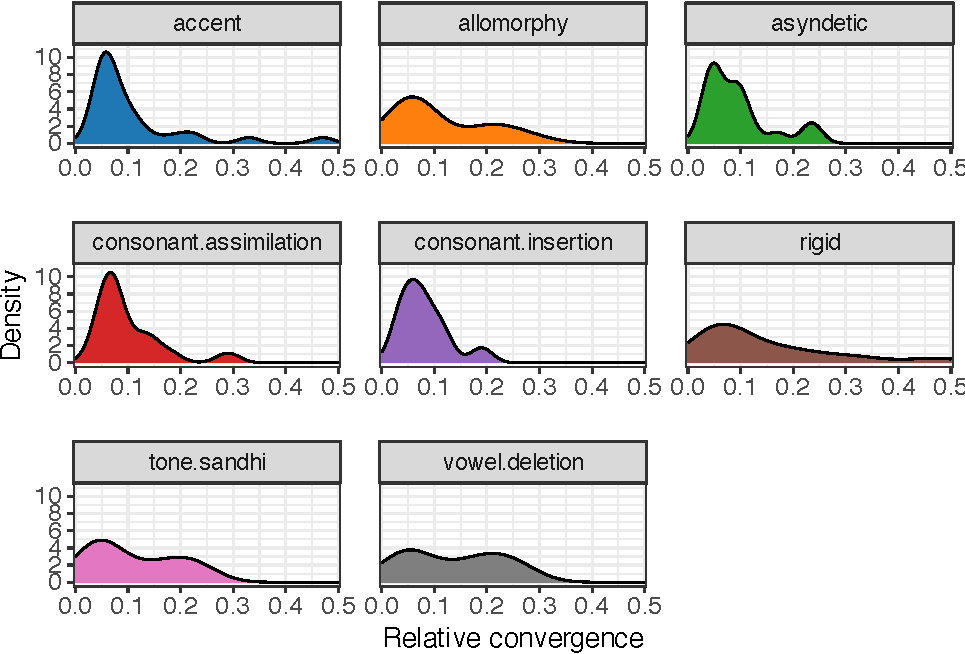
\includegraphics[width=0.9\textwidth,height=\textheight]{02_analyses_chapter17_files/figure-latex/dens crossl-1} \end{center}

\subsubsection{Random Forest analysis}\label{random-forest-analysis}

\section{Section 7}\label{section-7}

\subsection{Convergence and span size in phonological
domains}\label{convergence-and-span-size-in-phonological-domains}

To assess the word bisection thesis, i.e.~the idea that there are
phonological and grammatical words, we have a closer look at convergence
and span sizes in phonological vs.~morphosyntactic domains per language.
We first create the dataset by counting convergences per language with
relative span sizes.

\begin{Shaded}
\begin{Highlighting}[]
\CommentTok{\# count convergences between those domains per language}
\NormalTok{conv\_bisection }\OtherTok{\textless{}{-}}\NormalTok{ domains }\SpecialCharTok{\%\textgreater{}\%}
  \FunctionTok{unite}\NormalTok{(}\StringTok{"Spans"}\NormalTok{, Left\_Edge}\SpecialCharTok{:}\NormalTok{Right\_Edge, }\AttributeTok{sep =} \StringTok{"{-}"}\NormalTok{) }\SpecialCharTok{\%\textgreater{}\%}
  \FunctionTok{group\_by}\NormalTok{(Planar\_ID, Domain\_Type) }\SpecialCharTok{\%\textgreater{}\%}
  \FunctionTok{mutate}\NormalTok{(}\AttributeTok{Total\_Tests\_D =} \FunctionTok{n}\NormalTok{()) }\SpecialCharTok{\%\textgreater{}\%}
  \FunctionTok{group\_by}\NormalTok{(Planar\_ID, Domain\_Type, Spans) }\SpecialCharTok{\%\textgreater{}\%}
  \FunctionTok{mutate}\NormalTok{(}\AttributeTok{DConvergence =} \FunctionTok{n}\NormalTok{()) }\SpecialCharTok{\%\textgreater{}\%}
  \FunctionTok{ungroup}\NormalTok{()}

\CommentTok{\# with indeterminate = morphosyntactic}
\NormalTok{conv\_bisection\_lumped }\OtherTok{\textless{}{-}}\NormalTok{ domains }\SpecialCharTok{\%\textgreater{}\%}
  \FunctionTok{unite}\NormalTok{(}\StringTok{"Spans"}\NormalTok{, Left\_Edge}\SpecialCharTok{:}\NormalTok{Right\_Edge, }\AttributeTok{sep =} \StringTok{"{-}"}\NormalTok{) }\SpecialCharTok{\%\textgreater{}\%}
  \FunctionTok{mutate}\NormalTok{(}\AttributeTok{Domain\_Type\_Lumped =} \FunctionTok{if\_else}\NormalTok{(Domain\_Type }\SpecialCharTok{==} \StringTok{"indeterminate"}\NormalTok{, }\StringTok{"morphosyntactic"}\NormalTok{, Domain\_Type)) }\SpecialCharTok{\%\textgreater{}\%}
  \FunctionTok{group\_by}\NormalTok{(Planar\_ID, Domain\_Type) }\SpecialCharTok{\%\textgreater{}\%}
  \FunctionTok{mutate}\NormalTok{(}\AttributeTok{Total\_Tests\_DL =} \FunctionTok{n}\NormalTok{()) }\SpecialCharTok{\%\textgreater{}\%}
  \FunctionTok{group\_by}\NormalTok{(Planar\_ID, Domain\_Type, Spans) }\SpecialCharTok{\%\textgreater{}\%}
  \FunctionTok{mutate}\NormalTok{(}\AttributeTok{DLConvergence =} \FunctionTok{n}\NormalTok{()) }\SpecialCharTok{\%\textgreater{}\%}
  \FunctionTok{ungroup}\NormalTok{()}

\CommentTok{\# add back to df for plotting}
\NormalTok{domains\_bisection }\OtherTok{\textless{}{-}}\NormalTok{ conv\_bisection }\SpecialCharTok{\%\textgreater{}\%}
  \FunctionTok{left\_join}\NormalTok{(., conv\_bisection\_lumped) }\SpecialCharTok{\%\textgreater{}\%}
  \FunctionTok{mutate}\NormalTok{(}\AttributeTok{Relative\_DConvergence =} \FunctionTok{round}\NormalTok{(DConvergence }\SpecialCharTok{/}\NormalTok{ Total\_Tests\_D, }\DecValTok{2}\NormalTok{), }\AttributeTok{Relative\_DLConvergence =} \FunctionTok{round}\NormalTok{(DLConvergence }\SpecialCharTok{/}\NormalTok{ Total\_Tests\_DL, }\DecValTok{2}\NormalTok{))}
\end{Highlighting}
\end{Shaded}

We then plot the result for phonological domains.

\begin{Shaded}
\begin{Highlighting}[]
\CommentTok{\# plot lumped, phonological domains}
\NormalTok{plot\_points\_phon }\OtherTok{\textless{}{-}} \FunctionTok{ggplot}\NormalTok{(}\AttributeTok{data =} \FunctionTok{filter}\NormalTok{(domains\_bisection, Domain\_Type\_Lumped }\SpecialCharTok{==} \StringTok{"phonological"}\NormalTok{), }\FunctionTok{aes}\NormalTok{(}\AttributeTok{x =}\NormalTok{ Relative\_Size, }\AttributeTok{y =}\NormalTok{ DLConvergence)) }\SpecialCharTok{+}
  \FunctionTok{geom\_line}\NormalTok{(}\AttributeTok{linewidth =} \FloatTok{0.5}\NormalTok{) }\SpecialCharTok{+}
  \FunctionTok{geom\_point}\NormalTok{(}\AttributeTok{size =} \DecValTok{3}\NormalTok{, }\AttributeTok{color =} \StringTok{"darkorange2"}\NormalTok{) }\SpecialCharTok{+}
  \FunctionTok{facet\_wrap}\NormalTok{(}\SpecialCharTok{\textasciitilde{}}\NormalTok{Planar\_ID, }\AttributeTok{scales =} \StringTok{"free\_x"}\NormalTok{, }\AttributeTok{ncol =} \DecValTok{3}\NormalTok{) }\SpecialCharTok{+}
  \FunctionTok{labs}\NormalTok{(}\AttributeTok{x =} \StringTok{"Relative span size"}\NormalTok{, }\AttributeTok{y =} \StringTok{"Number of convergences"}\NormalTok{) }\SpecialCharTok{+}
  \FunctionTok{scale\_x\_continuous}\NormalTok{(}\AttributeTok{expand =} \FunctionTok{c}\NormalTok{(}\DecValTok{0}\NormalTok{, }\FloatTok{0.03}\NormalTok{), }\AttributeTok{breaks =} \FunctionTok{seq}\NormalTok{(}\DecValTok{0}\NormalTok{, }\DecValTok{1}\NormalTok{, }\FloatTok{0.25}\NormalTok{), }\AttributeTok{limits =} \FunctionTok{c}\NormalTok{(}\DecValTok{0}\NormalTok{, }\DecValTok{1}\NormalTok{)) }\SpecialCharTok{+}
  \FunctionTok{scale\_y\_continuous}\NormalTok{(}\AttributeTok{expand =} \FunctionTok{c}\NormalTok{(}\FloatTok{0.1}\NormalTok{, }\FloatTok{0.1}\NormalTok{)) }\SpecialCharTok{+}
  \FunctionTok{theme\_bw}\NormalTok{() }\SpecialCharTok{+}
  \FunctionTok{theme}\NormalTok{(}
    \AttributeTok{legend.position =} \StringTok{"top"}\NormalTok{,}
    \AttributeTok{legend.key.size =} \FunctionTok{unit}\NormalTok{(}\DecValTok{1}\NormalTok{, }\StringTok{"lines"}\NormalTok{),}
    \AttributeTok{legend.text =} \FunctionTok{element\_text}\NormalTok{(}\AttributeTok{size =} \DecValTok{11}\NormalTok{),}
    \AttributeTok{axis.text =} \FunctionTok{element\_text}\NormalTok{(}\AttributeTok{size =} \DecValTok{11}\NormalTok{),}
    \AttributeTok{axis.title =} \FunctionTok{element\_text}\NormalTok{(}\AttributeTok{size =} \DecValTok{13}\NormalTok{),}
    \AttributeTok{strip.text.x =} \FunctionTok{element\_text}\NormalTok{(}\AttributeTok{size =} \DecValTok{11}\NormalTok{),}
    \AttributeTok{panel.spacing =} \FunctionTok{unit}\NormalTok{(}\FloatTok{1.3}\NormalTok{, }\StringTok{"lines"}\NormalTok{),}
    \AttributeTok{strip.clip =} \StringTok{"off"}
\NormalTok{  )}
\NormalTok{plot\_points\_phon}
\end{Highlighting}
\end{Shaded}

\begin{center}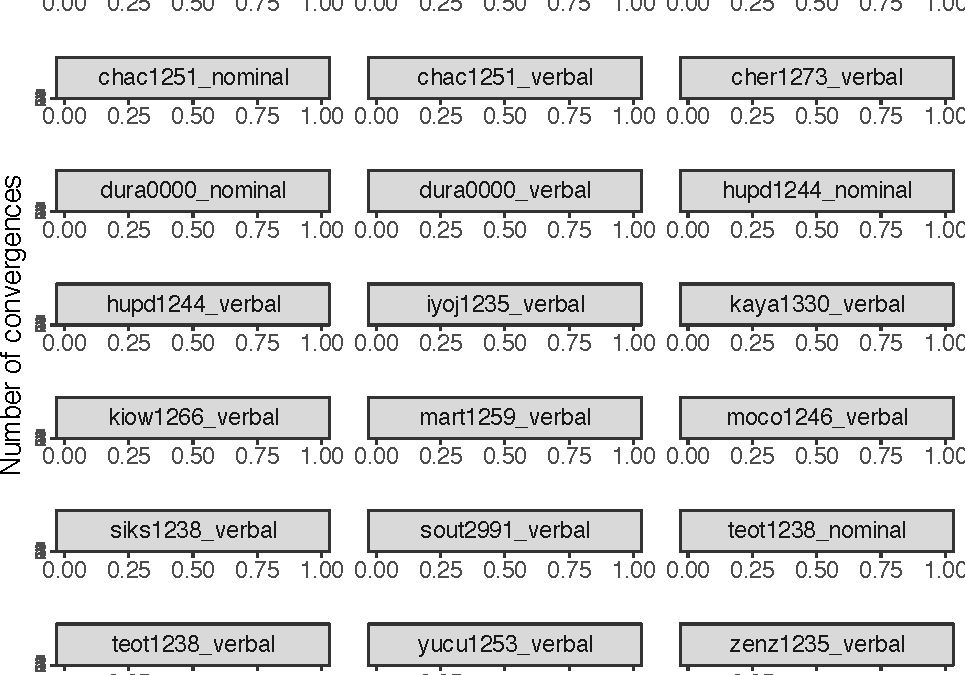
\includegraphics[width=0.9\textwidth,height=\textheight]{02_analyses_chapter17_files/figure-latex/conv phon plot-1} \end{center}

\subsection{Convergence and span size in morphosyntactic
domains}\label{convergence-and-span-size-in-morphosyntactic-domains}

And the same for morphosyntactic domains.

\begin{Shaded}
\begin{Highlighting}[]
\CommentTok{\# plot lumped, morphosyntactic domains}
\NormalTok{plot\_points\_ms }\OtherTok{\textless{}{-}} \FunctionTok{ggplot}\NormalTok{(}\AttributeTok{data =} \FunctionTok{filter}\NormalTok{(domains\_bisection, Domain\_Type\_Lumped }\SpecialCharTok{==} \StringTok{"morphosyntactic"}\NormalTok{), }\FunctionTok{aes}\NormalTok{(}\AttributeTok{x =}\NormalTok{ Relative\_Size, }\AttributeTok{y =}\NormalTok{ DLConvergence)) }\SpecialCharTok{+}
  \FunctionTok{geom\_line}\NormalTok{(}\AttributeTok{linewidth =} \FloatTok{0.5}\NormalTok{) }\SpecialCharTok{+}
  \FunctionTok{geom\_point}\NormalTok{(}\AttributeTok{size =} \DecValTok{3}\NormalTok{, }\AttributeTok{color =} \StringTok{"dodgerblue3"}\NormalTok{) }\SpecialCharTok{+}
  \FunctionTok{facet\_wrap}\NormalTok{(}\SpecialCharTok{\textasciitilde{}}\NormalTok{Planar\_ID, }\AttributeTok{scales =} \StringTok{"free\_x"}\NormalTok{, }\AttributeTok{ncol =} \DecValTok{3}\NormalTok{) }\SpecialCharTok{+}
  \FunctionTok{labs}\NormalTok{(}\AttributeTok{x =} \StringTok{"Relative span size"}\NormalTok{, }\AttributeTok{y =} \StringTok{"Number of convergences"}\NormalTok{) }\SpecialCharTok{+}
  \FunctionTok{scale\_x\_continuous}\NormalTok{(}\AttributeTok{expand =} \FunctionTok{c}\NormalTok{(}\DecValTok{0}\NormalTok{, }\FloatTok{0.04}\NormalTok{), }\AttributeTok{breaks =} \FunctionTok{seq}\NormalTok{(}\DecValTok{0}\NormalTok{, }\DecValTok{1}\NormalTok{, }\FloatTok{0.25}\NormalTok{), }\AttributeTok{limits =} \FunctionTok{c}\NormalTok{(}\DecValTok{0}\NormalTok{, }\DecValTok{1}\NormalTok{)) }\SpecialCharTok{+}
  \FunctionTok{scale\_y\_continuous}\NormalTok{(}\AttributeTok{expand =} \FunctionTok{c}\NormalTok{(}\DecValTok{0}\NormalTok{, }\FloatTok{0.3}\NormalTok{)) }\SpecialCharTok{+}
  \FunctionTok{theme\_bw}\NormalTok{() }\SpecialCharTok{+}
  \FunctionTok{theme}\NormalTok{(}
    \AttributeTok{legend.position =} \StringTok{"top"}\NormalTok{,}
    \AttributeTok{legend.key.size =} \FunctionTok{unit}\NormalTok{(}\DecValTok{1}\NormalTok{, }\StringTok{"lines"}\NormalTok{),}
    \AttributeTok{legend.text =} \FunctionTok{element\_text}\NormalTok{(}\AttributeTok{size =} \DecValTok{11}\NormalTok{),}
    \AttributeTok{axis.text =} \FunctionTok{element\_text}\NormalTok{(}\AttributeTok{size =} \DecValTok{11}\NormalTok{),}
    \AttributeTok{axis.title =} \FunctionTok{element\_text}\NormalTok{(}\AttributeTok{size =} \DecValTok{13}\NormalTok{),}
    \AttributeTok{strip.text.x =} \FunctionTok{element\_text}\NormalTok{(}\AttributeTok{size =} \DecValTok{11}\NormalTok{),}
    \AttributeTok{panel.spacing =} \FunctionTok{unit}\NormalTok{(}\FloatTok{1.3}\NormalTok{, }\StringTok{"lines"}\NormalTok{),}
    \AttributeTok{strip.clip =} \StringTok{"off"}
\NormalTok{  )}
\NormalTok{plot\_points\_ms}
\end{Highlighting}
\end{Shaded}

\begin{center}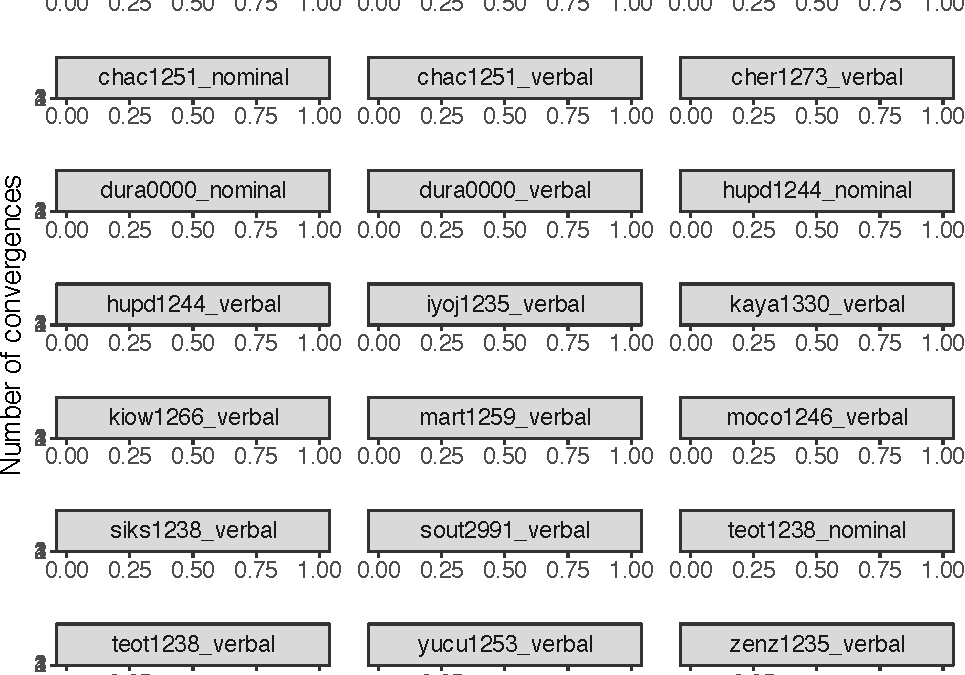
\includegraphics[width=0.9\textwidth,height=\textheight]{02_analyses_chapter17_files/figure-latex/conv morph-1} \end{center}

\section*{References}\label{references}
\addcontentsline{toc}{section}{References}

\phantomsection\label{refs}
\begin{CSLReferences}{1}{0}
\bibitem[\citeproctext]{ref-kahle2013ggmap}
Kahle, David \& Wickham, Hadley. 2013. Ggmap: Spatial visualization with
ggplot2. \emph{The R Journal}.
\url{https://journal.r-project.org/archive/2013-1/kahle-wickham.pdf}
5(1). 144--161.

\end{CSLReferences}

\end{document}
